%!TEX root = ../risk_report.tex

%!TEX root = ../risk_report.tex

\chapter{\emph{Risk} in health articles in the NYT}

\vspace{5mm}
\noindent\begin{tcolorbox}[colback=yellow!5,colframe=yellow!40!black,title=Forthcoming chapter]
\parbox{1\textwidth}{%
This chapter of our report is taken from a forthcoming book chapter: \\ 

Zinn, J. O. \& McDonald, D. (2015). \emph{Changing Discourses of Risk and Health-Risk: a corpus analysis of the usage of risk language in The New York Times}. Chamberlain, M. (ed.) 2015/6: Medicine, Discourse, Power and Risk. Routledge.}
\end{tcolorbox}
\vspace{5mm}

\section*{Abstract}

In recent decades the increasing digitisation of newspaper archives has opened new opportunities for the social sciences to examine social change. This is of particular interest for the sociology of risk and uncertainty, where different approaches compete to explain historical social transformations. This chapter reports results from an ongoing research project that examines longitudinal changes in risk reporting in print news media by the example of The New York Times (NYT). It has two major purposes. Firstly, we aim to demonstrate the usefulness of techniques from corpus and computational linguistics as means of examining how social change may be reflected in print news media. Secondly, we aim to examine a number of hypotheses from common sociological theories. Here, we show that there is good evidence for the increasing institutionalisation of risk practices in a growing number of social domains. Analysing language use in approximately 150,000 articles spanning the past 28 years, we find empirical support for the individualisation of risk, for a growing possibilistic approach to risk, and for decreasing agency in risk discourses. Focussing specifically on health-related articles, we uncover evidence for the growing salience of non-infectious diseases, and for an increase in the frequency with which health, risk and science and technology discourses co-occur. We conclude with perspectives for further research.

%Keywords 

%social change; corpus linguistics; discourse; print news media; New York Times; systemic functional linguistics; 

\section{Introduction}

In recent decades, with the development of social media, mobile devices and advancements in the digitisation and storage of text, Big Data are offering new opportunities for social science research. It is not only the production of new data in the present, but the digitisation of old data such as (historical) newspaper archives, which open unprecedented opportunities for sociologists to examine long-term social change. This is of particular interest for the sociology of risk and uncertainty, where different approaches compete to explain social change towards risk. Though the cultural approach (Douglas 1990, 1992; Douglas \& Wildavsky 1982), the risk society perspective (Beck 1992, 2009; Giddens 1990, 2000), governmentality (Ewald 1986; Dean 1999; Rose 1999; O'Malley 2004), and modern systems theory (Luhmann 1989, 1993) have all made significant contributions describing social risk phenomena, there have been few attempts to examine the relative explanatory power of different approaches for an overall shift towards risk in public debates or how different social domains and events have contributed to the dynamics of societal risk discourse. 

This is surprising, given that the media have been identified as crucial for social risk awareness. Many risks are only experienced through the reporting in the media. They might happen at different places or require research to be identified. Therefore, the media shape societal risk awareness. At the same time, the media report on issues considered relevant and thereby reflect typical social issues at the time and how they are understood. Language is a key element in this process. How a risk is reported, which words and grammatical constructions are used reflect a deeper social reality, expresses a particular Zeitgeist, institutional set up and socio-cultural context. 

Our study capitalises on the increased availability of digitised newspaper archives, in order to examine discursive changes in the meaning and use of risk, focussing on data from \emph{The New York Times} (NYT) between 1987---2014. In contrast to most risk studies, we do not examine a particular risk but how the risk semantic---or more concretely---how risk as a lexical item occurs, in which forms and in which contexts. We make use of a combination of corpus linguistic methods and systemic-functional linguistic theory (Halliday \& Matthiessen, 2004) to analyse the lexical and grammatical patterns in clauses containing a risk word, identifying key areas of change.

This chapter has two purposes. Firstly, we aim to demonstrate the viability of corpus linguistic methods as a means of empirically observing longitudinal change in risk discourse. Secondly, we test some key hypotheses in risk research. 

We begin our contribution with the proposition that examining the use of the term risk in media coverage can be a useful approach to understand long-term social change and the explanatory power of different social science approaches to risk. Next, we outline a number of key hypotheses from risk theories more generally, and for the health domain in particular, considering how these hypotheses might manifest in language. We then outline the methodological foundations of our study, which utilises systemic functional linguistics and frame semantics' conceptualisation of the 'risk frame' as a theoretical framework, and practices from corpus and computational linguistics as an approach to data analysis. In the results, we show that the growing institutionalisation of risk practices can be clearly found in changing linguistic forms. Among other findings, we demonstrate that there is a clear trend towards the negative side of risk, and, increasingly, a representation of risk as uncertain rather than controlled. Everyday people are increasingly presented as bearers of risk, while powerful institutions and actors remain the most common risk takers. Furthermore, we highlight the strong relationship of risk and health-related news in particular. This is evidenced by very high peaks in the co-occurrence of risk and single health-related events and\slash or ongoing health issues such as chronic illnesses or cancer. Also within the area of health risks, we find an increase in reference to scientific research and experts. We finish with concluding remarks highlighting some key issues and perspectives for further research.

\section{State of research and some key questions}

Mainstream social science theories conceptualise `risk' relatively independent of empirical linguistic evidence. For example, Douglas does not emphasise the difference of a risk discourse compared to danger or threat. Instead she outlines the functional equivalence of earlier notions of sin and taboo compared to the modern notion of risk. From this perspective, risk becomes synonymous with danger; more risk would equate to more danger (Douglas 1990, Lupton 1999). She argues that risk and danger respectively were transformed through socio-cultural worldviews into challenges for a particular institutional set up of a social unit. 

In the governmentality perspective, risk has often been associated with calculative technologies. In many studies, reference is made to the application of technical or formal techniques such as probability analysis and statistics, which usually use risk as a technical or jargon term, rather than threat or possible harm or danger. Ewald suggested when discussing insurance that a risk becomes only a risk through being part of a statistic probabilistic calculation (Ewald 1991). Bernstein (1997) has shown that risk as a concept is linked to the development and application of statistics in different areas of society, as Hacking (1990, 1991) has argued, risk has been central in new ways of governing populations. At the same time, scholars emphasise the importance of the normative contexts, which determines how calculative technologies are set up and used in social practice. Scholars in the governmentality perspective often emphasise the influence of neoliberalism for the pervasiveness of risk discourse (Dean 1999; Rose 1999; Kelly 2006). More generally Kemshall (2002) observed an increased responsibilisation of the individual in institutional practices in the UK while Hacker (2006) stated The Great Risk Shift from social institutions to the individual in the US. 

In contrast to the partly rather `technical' understanding of risk in the governmentality perspective, Luhmann, in his analysis of social structure and semantics, has claimed, that the risk semantic stands for a historical new social experience that required a new expression (1993: 10\slash 1): 

`Certain advantages are to be gained only if something is at stake. ... It is a matter of a decision that, as can be foreseen, will be subsequently regretted if a loss that one had hoped to avert occurs.'

However, Luhmann's argument mainly refers to the shift from stratified differentiation in the Middle Ages to functional differentiation in modern industrialised societies. Beck, instead, claims that the more recent increase of risk communication would be a result of a shift within modernisation in particular after WW2. 

According to Beck, the significant increase of risk in public debates would be the result of the unexpected side effects of modernisation that had produced new risks, uncertainties and new unknown spheres in contrast to the modern myth of increasing control and predictability (e.g. Weber 1948). As a result of difficulties in controlling and predicting events in the natural and social world (even the distinction between both becomes questionable) the modern myth of increased rationality has been challenged. However, the erosion of scientific authority caused by the lacking ability to solve social conflicts through the provision of true knowledge has not lead to a loss of importance of scientific expertise. Instead, Beck claims that science has become even more significant to strengthen one's argument (1992). Scientific expertise is still a crucial resource in social claims making processes and is still one of the most trustworthy sources in particular the media rely on. 

In Beck's view, the increasing worries about risk and uncertainty would be caused by the quality of new risks and mega-risks (Beck 1992, 2009) but also processes of institutional individualism linked to de-traditionalisation (Beck 1992, Beck \& Beck-Gernsheim 2002). The assumption is that traditions and old institutions would lose their power to guide decision-making and to protect against risks. Individuals would increasingly have to make decisions and to reinvent themselves in a context of decreasing control and predictability. The freedoms we gain from detraditionalisation would be replaced by risks and uncertainties to be dealt with individually. Late or reflexive modernity would be characterised by the risky freedoms, which expose individuals to new decision making situations. Some scholars claim that in particular people in powerful positions and the privileged middle class is among the individualisation winners while many are among the individualisation losers being mainly made responsible for what happens to them without much opportunity to plan their life (Beck \& Beck-Gernsheim 2002: 47). 

While there is a plethora of empirical risk studies addressing a large number of risk issues, there is comparatively little work which reconstructs particular risk issues in a long term perspective such as the introduction of social insurance in France (Ewald 1986), the introduction of life insurance in the US (Zelizer 1983), the development of environmental risk debates (Strydom 2002), or the shift from danger to risk in psychiatry (Castel 1991). 

There is also little research that systematically examines how different areas relate to each other or to what extent particular social domains contribute to the general risk awareness and\slash or public discourses. Many media studies refer to particular risk issues or relatively short periods of attention cycles in media coverage when examining the dynamics of risk discourses in the media (Grundmann et al. 2013; Holland et al. 2012). They often refer to a particular risk such as climate change, infectious disease or a new technology and distinguish positive from negative or supportive and critical discourses or reconstruct dynamics of risk reporting (Grundmann \& Krishnamurthy 2010; Grundmann \& Scott 2014, Holland et al. 2012). 

There is very little work in the vein of Mairal (2011), who examines more generally how past experiences with risk influence and structure the ways in which we think about unknown and uncertain risks of the future. A good example is how the so called swine flu (H1N1) in 2009 was perceived against the background of the deadly Spanish flu pandemic from 1918 to 1920, which killed more than estimated 50 million people worldwide.

Mairal's research also developed an interesting argument about the development of a particular genre in journalism that places risk in its centre. He used Defoe's work on the Plague in London in 1665 as a case study to show how an emerging practice of evidence-based reporting developed into a new `narrative matrix' that remains dominant in the reporting of risk in mass media today.

If risk is part of a particular new genre of journalism, Skolbekken's observation of a risk epidemic in scholarly articles in medical journals in the US, Britain and Scandinavia from 1967 to 1991 might be crucial for understanding increased usage of the risk semantic in the health area. He suggests that the shift towards risk cannot be explained by a change in terminology only and hypothesises that the shift results from a particular social culture that developed historically and is linked to the development of probability statistics, focus on risk management and health promotion and computer technology. However, he does not provide evidence how the risk epidemic connects to public discourse. 

Coming from a discourse studies perspective, in recent decades, applied linguists have become interested in incorporating sociological dimensions into the study of language (e.g. Van Dijk 1997, Wodak \& Meyer 2001). To date, however, this stream of research has contributed little to the reconstruction of the historical development of discourses (Brinton 2001; Harding 2006; Carabine 2001) although many linguists are interesting in examining long-term semantic changes (e.g. Nerlich \& Clarke 1988, 1992, 2000; Traugott \& Dasher 2002). 

Regarding risk, corpus linguists have shown that sociologists' assumptions about the usage of risk are often informed by everyday life knowledge rather than systematic empirical analysis of how the term risk is actually used (Hamilton et al. 2007). Frame Semantics (Fillmore \& Atkins 1992) has provided a detailed analysis of the available risk-frames; but neither approach examines historical changes of the usage and notion of risk.

\section{Towards a usage-driven account of risk}

It is not clear what the relationship between linguistic changes in the media and broader institutional and socio-structural changes are. In media studies, there is vast research on agenda-setting studies (grounded in the traditional media effects tradition) that explores the relationships between the media and the public agendas (e.g. McCombs \& Shaw 1972; McCombs 2004). Yet there are very few studies which systematically examine what forces set the media agenda (one exception: Collistra 2012) and how the media agenda is influenced by broader societal developments or how more general historical ideas (Koselleck 1989) influence and change media coverage. 

Conceptualisations of language change within linguistics and history have tended to focus more on broader social movements than on the role played by single events. The recent emergence of large, well-structured digital datasets, as well as tools and methods capable of analysing them, however, makes such studies possible, both on the scale of evolution of jargon terms within a single online community (Danescu-Niculescu-Mizil, 2013) to research utilising Google's database of millions of digitised books, chronologically arranged (Michel et al, 2011).

In a discourse analytic perspective, a contrasting argument would emphasise that we can only change a future in a particular way when we can imagine that the future is different from the past. Or, we could say that a society always produces discourses about more possible futures than can be realised (Luhmann 1980). This implies that thinking and talking about possible futures might change discursive practices even before institutional changes manifest.

\section{Significant increase of the usage of risk in the NYT after WW2}

Previous research (Zinn 2010) has proven that the increasing usage of the term risk in media coverage of NYT is one of the most outstanding developments compared to similar phrases after WW2. Figure \ref{fig:num_with_token} shows the number of articles where risk and other related words such as threat or danger were mentioned at least once. Danger has significantly decreased after WW2 while threat became common during the Great Depression and since then remained on a relatively stable level. Only recently, after September 11 and the Iraq War, the number of articles using threat again increased in usage. Risk had a turbulent trajectory after WW2 with no clear direction but with the late 1968s and early 1970s the trajectory is a steep increase where major disasters as Chernobyl and the terror attack of September 11 were preceded by an increase in risk communication in the NYT.

The preceding increase of articles using risk language shows that already before these iconic events happened, social risk communication had increased, which might imply a heightened social sensitivity for risk issues before these disasters took place. We take this as a first indication how the analysis of large collections of digitised text might be able to discover unexpected insights into risk. That said, we can draw only limited conclusions from this kind of data, as it provides little possibility of discovering the co-text and context in which risk and related words appear.

\begin{figure}[htb!]
\centering
\addvbuffer[12pt 0pt]{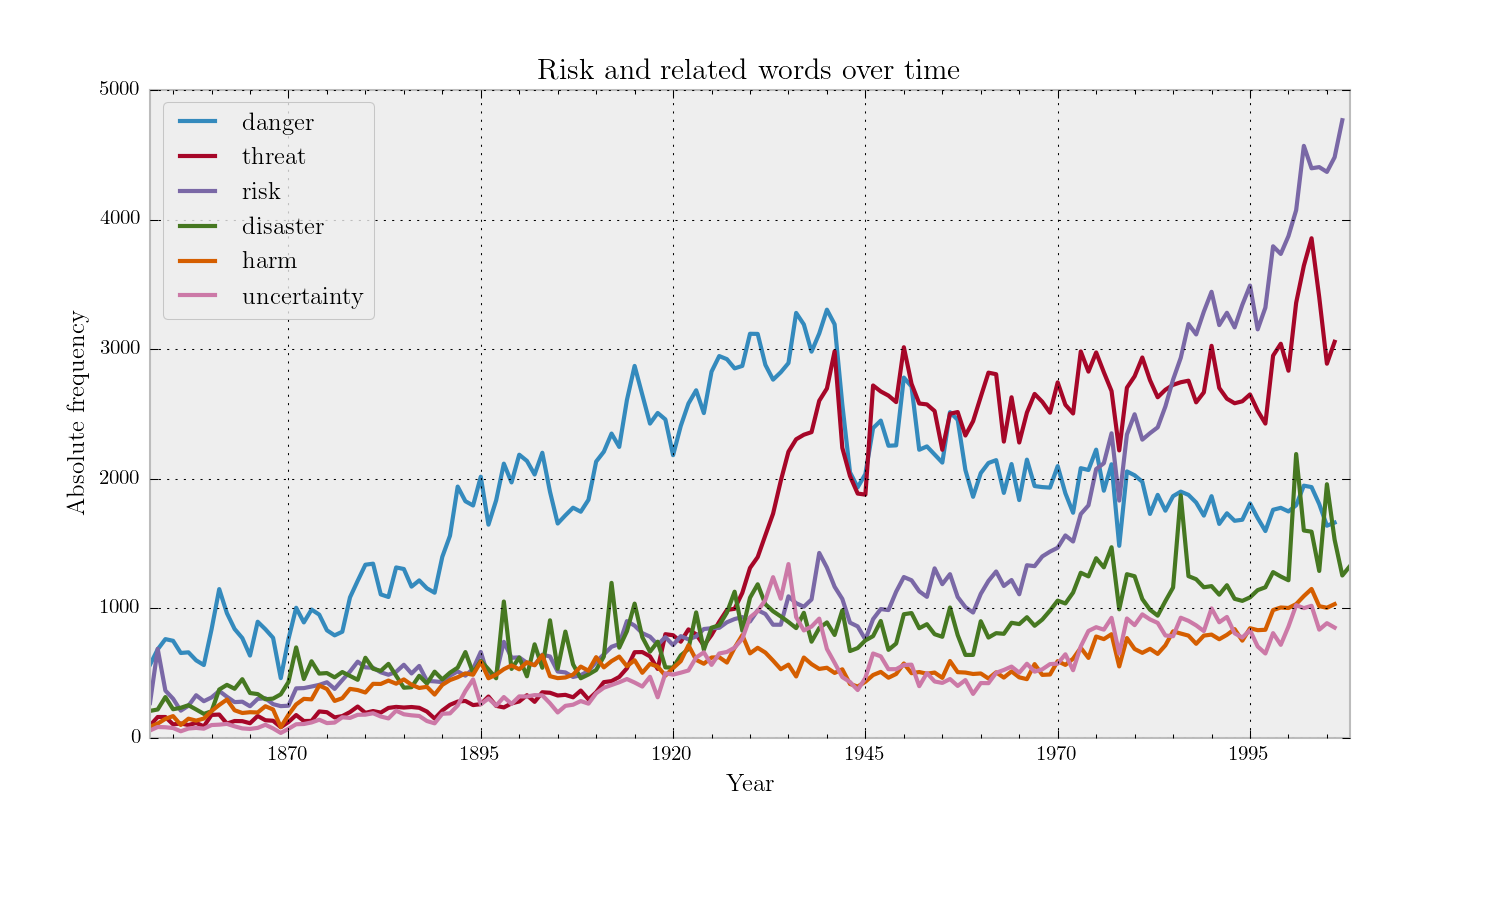
\includegraphics[width=0.75\textwidth]{../images/risk_related_june_colour}}
\caption[Number of articles with at least one risk token, 1852--2008]{Number of articles in The New York Times with at least one risk token, 1852--2008 (source: Zinn 2010)}
\label{fig:num_with_token}
\end{figure}

\section{Hypotheses: general trend towards risk}

Many scholars claim that there is a strong tendency towards negative connotations of risk, and an increasing synonymy with words denoting negative outcomes, such as danger or harm (Douglas 1992; Lupton 1999). Risk less and less refers to the risk taking process, which involves opportunities as well as possible negative outcomes. Public debates about risk would increasingly focus on the negative side only, the possible dangers and threats. Linguistically, evidence for increasing synonymy of risk and negative outcomes could be observed by looking at the functional role of risk words: when risk is a participant in discourse (`The risk was real'), synonymy with negative outcomes is greater than when risk is a process (`They risked their safety'). This can be demonstrated by contrasting risk in both roles with explicit positive outcomes

\begin{enumerate} [before=\color{black}\ttfamily] \setlength\itemsep{0em} \small
\item The risks outweighed the rewards; the risk\slash benefit ratio
\item He risked alienating voters, but it paid off
\item The risks had rewards
\end{enumerate}

Note that in process-range configurations, though risk is nominal, it conforms semantically to the role of process, rather than participant:

\begin{enumerate} [before=\color{black}\ttfamily] \setlength\itemsep{0em} \small
\item They ran\slash took the risk and were rewarded
\end{enumerate}

For example, Beck (1992) has claimed that risk would increasingly escape individual control. They cannot be calculated. Instead, we now have to deal with the experience of possible risks---the general worry that things go wrong or what might happen to us---rather than with the notion of calculated risks indicating that risks are under control. Reporting that has an increasingly possibilistic approach to risk would support his claim of increased concerns about risk. Linguistically, calculatedness of risk could be examined by locating the kinds of modifiers of nominal risks (`A calculated\slash potential risk').

At the same time different approaches in risk studies (e.g. Beck 1992, Dean 1999) have in different ways emphasised a shift towards greater responsibility of the individual reflecting other US scholars who have criticised growing individualism in the USA (Slater 1970; Putnam 2000), which has also manifested in a recent institutional risk shift of responsibility in public and social policy towards the individual (Hacker 2006). We expect that such a shift would be detectable in the NYT through, for example, a stronger mentioning of everyday life people rather than social institutions and organisation in relation to risk.

\section{The centrality of the health sector in driving public risk debates}

When risk research developed within sociology in the 1980s the focus was mainly on new technologies and in particular nuclear power (Douglas \& Wildavsky 1982, Perrow 1984, Luhmann 1989, Beck 1992). However, there had also been indications that risk thinking is entering society on different levels and in different areas. In particular, Skolbekken had indicated a shift towards risk in health in his article about a risk epidemic in medical science journals though not examining to what extent the scientific debates have entered public debates and news media. 

\begin{figure}[htb!]
\centering
\addvbuffer[12pt 0pt]{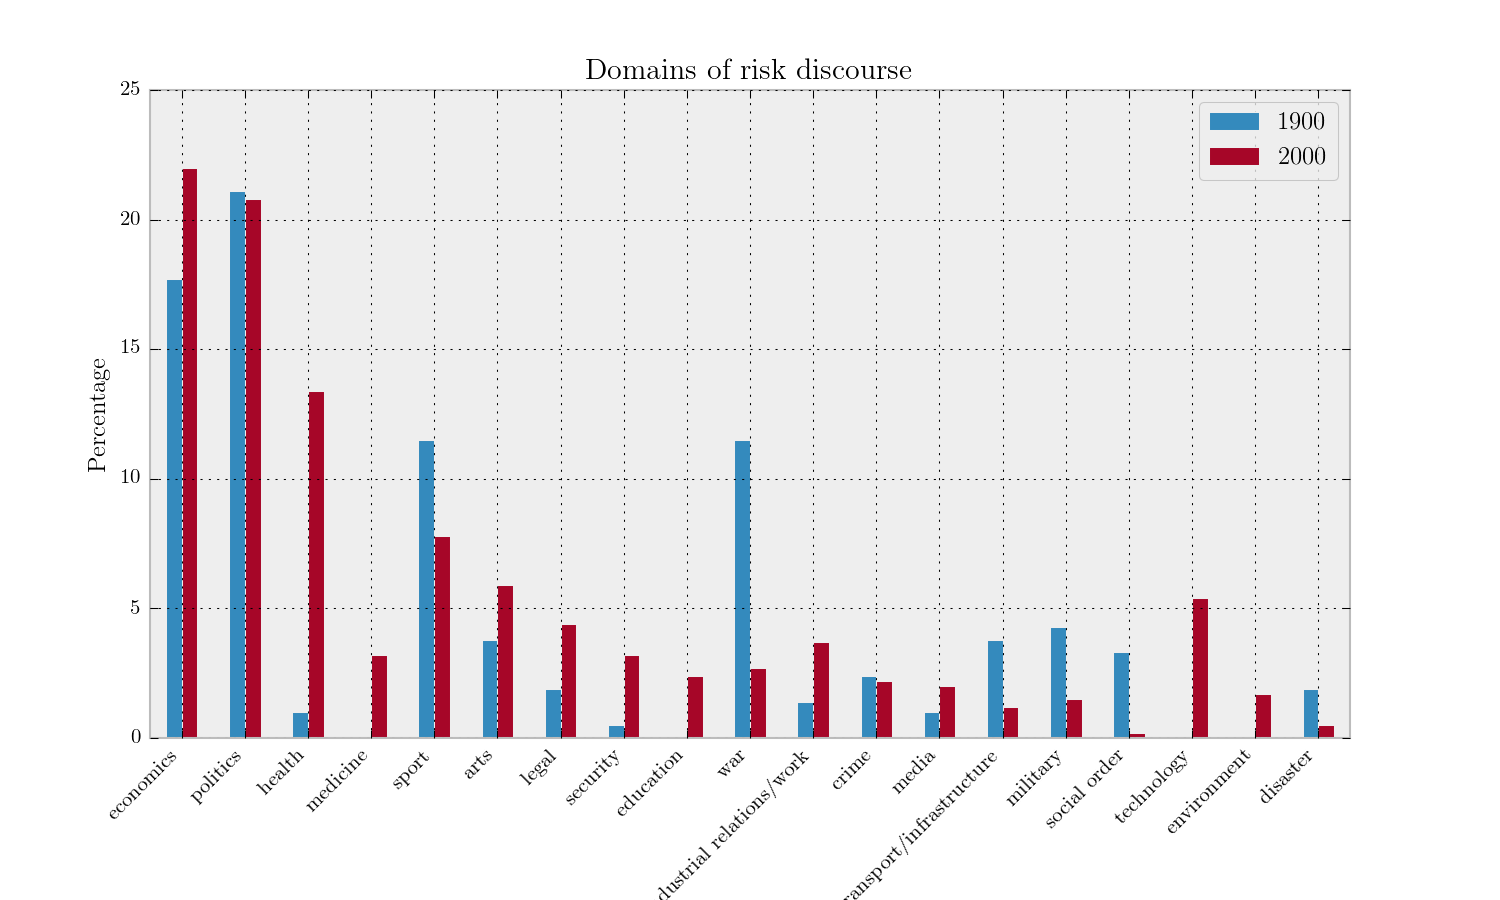
\includegraphics[width=0.75\textwidth]{../images/domains_june_colour}}
\caption[Number of articles containing at least one risk token by topic]{Number of articles in The New York Times containing at least one risk token by topic\slash domain, 1900 versus 2000 (source: Zinn 2011)}
\label{fig:rdomains}
\end{figure}

In order to get a better feeling for the relative relevance of risk in different social domains Zinn (2011) conducted an explorative study in which he compared the news coverage in the volume 1900 with 2000 of the New York Times to see to what extent reporting using the risk semantic has changed historically. The study took samples from the 1900 volume (n=209; N=622) and the 2000 volume (n=409; N=5188). The areas were thematically coded regarding the domains they are referring to. For example, technological risks referred to risks which were caused by at the time relatively new technologies. Health refers to health issues more generally while medicine refers to organised\slash institutionalised medicine. Similarly reporting on war is distinguished from reports on the military as an organisation (Zinn 2011). Assuming that what is newsworthy reflects to a large extent the reality of a society at a particular time and not only a specific mode of news production seems supported by the areas connected to risk in the earlier volume compared with the later (e.g. the stronger prominence of war, the military, transport\slash infrastructure, social order, and disaster; compare Figure \ref{fig:rdomains}). It supports the recent occurrence of risk in the context of new technologies and the environment but it also shows the outstanding importance of health and medicine as sectors of risk discourses in the media. It indicates that the risk semantic entered increasingly a broader range of different social domains in the more recent volume and draws attention to often-neglected areas in societal risk debates, such as sport and arts. If confirmed by more rigorous research, the picture drawn by this exploration suggests placing health related issues more centrally in theorising on a recent shift towards a risk society. 

\section{Hypotheses: health domain}

There are a number of assumptions about developments in the area of health and illness that have not yet been examined empirically. There is a well-known general trend of civilisation illnesses and chronic illnesses becoming more dominant in health and illness while infectious diseases lose relative importance but do not disappear (e.g. Kury\l{}owicz \& Kopczy\'{n}ski 1986). Our interest is in how such trends are reflected in the usage of the risk semantic in the health domain.

A number of scholars have claimed scientific research entering news reporting (Mairal 2011), the importance of research for claims making (Beck 1992) while Skolbekken (1995) has found a risk epidemic in health journals in the US medical journals, among others. Therefore we sought to determine whether the increasing usage of the risk semantic in news coverage is indeed increasingly referring to scientific studies and experts.

We also wanted to test whether the trend towards individualism (Beck 1992; Putnam 2000) manifests in issues reported in the health domain. It was of interest, for example, what role common terms for people in everyday life (woman, man, person, child, etc.) played in the landscape of risk, and how this differed from the role played by institutions or influential people.

\section{Methodology and Methods}

There is no doubt that the media and newspaper coverage is an important part of social reality, constituting an arena for social discourses and influencing individual comprehension (e.g. Pidgeon et al. 2003; Flynn et al. 2001; Gamson 1989; Stuart et al. 2000). This happens simultaneously on the content plane of discourse-semantics, and on the expression plane of lexis and grammar. For example, functional linguistic theories such as frame semantics and systemic functional linguistics support the view that social changes and language changes are connected and assume that meaning can be made only with reference to a structured background of experience, beliefs, or practices (Fillmore \& Atkins 1992, Halliday \& Matthiessen, 2004). 

Since media coverage relies on the social knowledge and language of a society, it contributes to and reflects changes in social symbols, norms, values and institutions. Thus, media coverage can be used to examine social change, although there are some restrictions. The media follows a specific logic of news-production and risk-management strategies. Changes in the readership, the ideological stance and the specific socially stratified audience may influence results (Kitzinger 1999; Boyne 2003, p. 23-41) and have to be carefully controlled by analysis of changes in the organisational context of the NYT (e.g. changes in leadership, publisher and editors, corporate identity) and its position in the history of US journalism. 

The Glasgow approach in media studies has emphasised the need to research the media production process in much more detail. However, the study approaches the risk semantic from a different perspective. It is informed by the sociology of risk, sociological analysis of historical social change, discourse analysis and corpus linguistics. 

From a media studies perspective, the argument supported by F\"{u}rsich (2009) for text-focused analysis of media discourses comes closest to our approach. This perspective interprets the text as a structure produced in complex processes, which involve a range of players, including journalists, readerships and media moguls, and open a number of different, but not arbitrary, interpretations. It is unlikely that the power struggle in a newspaper's management or a shift in journalism can fully determine the usage of a specific semantic, even in democratic countries with a relatively independent press (Tulloch \& Zinn 2011). Far more reasonable is the assumption that the instantiation of particular discourses in news plays a role in both the construction and reflection of more general social changes. Considering these concerns an explorative examination of possible differences in news coverage of the NYT and the Washington Post supports this assumption (Zinn 2010, p. 115). Only relatively minor differences in the number of articles using `risk' but very similar long-term developments were found. Thus we assumed that the long-term historical changes are sufficiently general (Koselleck 2002; Luhmann 1980) that they can be traced even through a single newspaper. 

In the following we outline the risk-frames identified by Fillmore and Atkins (1992, p. 76f.) we use as a starting point for understanding the kinds of participant roles in the process of risking. We then outline our use of systemic functional linguistics for our analyses.

\subsection{Risk in Frame Semantics}

Frame semantics can serve as a general blueprint to understand the common risk frame in use. Developed through the analysis of a large text corpus it is claimed to represent the complete structure of the risk frame. This includes an actor, a valued object, a goal, a deed, possible harm and a victim, which may not necessarily be the actor (see Figure \ref{fig:fil_atk}).

%\begin{figure}[htb!]
%\centering
%\addvbuffer[12pt 0pt]{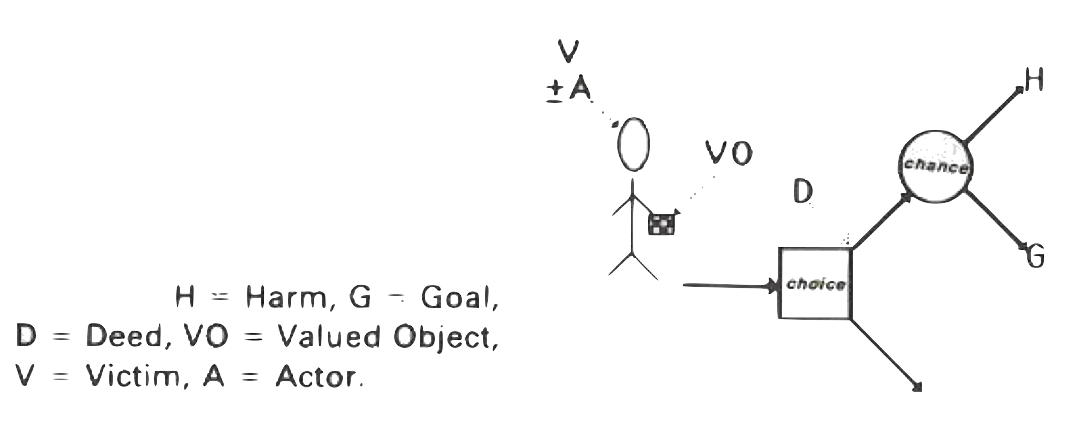
\includegraphics[width=0.75\textwidth]{../images/riskframe}}
%\caption[Risk Frame]{Risk Frame (from Fillmore \& Atkins, 1992)}
%%\label{fig:comparison}
%\end{figure}


Hamilton et al. (2007) use a frame semantics approach to understand the behaviour of risk in two corpora: the 56 million word \emph{Collins WordbanksOnline Corpus} and the five million word CANCODE. They find that risk is commonly nominal in contemporary language use, and that risk co-occurs with  negative semantic prosody. Further, they find that health risks are a more salient semantic domain in than has been commonly understood in risk research.

We depart from their methods in a number of respects, however. First, they use general corpora, while we used a specialised corpus of NYT articles. Second, our study is diachronic, while theirs is largely monochronic. Third, we differ dramatically in the number of risk words analysed (approx. 300 vs. 240,082). Fourth, they relied on collocation, while we parsed the data for linguistic structure and performed specific queries of the lexicogrammar of clauses containing risk words. Finally, we augment the frame-semantic approach to risk with core tenets of systemic-functional grammar. Though the components of the risk frame are semantically clear, they are often difficult to automatically extract from corpora, even when the corpus has been annotated for grammatical structure: even in prototypical risk processes, whether or not the valued object or the possible harm is often grammatically unmarked (I risked my life\slash I risked death). When risk is a modifier, or a participant, things become less clear still, with fewer of the components of the frame being mentioned overtly at all. Furthermore, when risk is not the process or participant, the extent to which the risk frame is being instantiated is difficult to assess:

\begin{enumerate} [before=\color{black}\ttfamily] \setlength\itemsep{0em} \small
\item In 1999, we sold the company, and the next year, we moved to the United States with our two children---a third was born in 2003---so I could pursue my idea of helping low-income, at-risk youth. 
\item Mr. Escobedo said that Vioxx was especially dangerous to Mr. Garza because of his other risk factors and that he should never have been prescribed the drug.
\end{enumerate}

\subsection{Systemic functional linguistics and the systemic-functional grammar}

We utilise systemic functional linguistics as both an English grammar and a means of connecting lexical and grammatical phenomena to their meaning and function in news discourse. Unlike frame semantics, it is not a cognitive-semantic theory, instead prioritising lexis and grammar as delicate meaning-making resources, and arguing that context is often embedded within the linguistic choices made in a text \cite{eggins_introduction_2004}. These ideas are particularly helpful affordances in analyses of texts within a one-way medium such as print news, especially in diachronic contexts, where access to writers and readers for follow-up interviews is extremely limited.

In systemic functional linguistics, the transitivity system is considered the means through which experiential meanings are made---that is, meanings designed to represent events and happenings in the social world (as opposed to the Mood system, which is responsible for the negotiation of interpersonal meanings). It is here that we situate our analysis of risk (though forthcoming work provides a treatment of risk according to Mood choices too).

Within the transitivity system, the three main functional roles are participant, process and circumstance. These roles pattern to some extent with formal word classes. Verbs and verb phrases congruently represent processes. Nouns and noun phrases typically represent participants, and prepositional phrases and adverbs typically represent circumstances. The example shown in Figure \ref{fig:transannotation} shows a basic transitivity analysis of a clause from our data with the heads of the participants and process in bold.

%\begin{figure}[htb]
%\centering \small \onehalfspacing
%\begin{tabularx}{0.75\textwidth}{|l|l|X|X|X|}
%\hline
%\emph{But}     & \emph{the bang of the gavel}             & \emph{can hold}          & \emph{risk} & \emph{for novices}          \\ \hline
%~ & Participant: & Process: & Participant: & Circumstance:  \\
%~ & Carrier & Relational \mbox{attributive} & Attribute &  Extent \\ \hline
%\end{tabularx}
%\caption{Transitivity analysis of a clause}
%\label{fig:transannotation2}
%\end{figure}

Using these categories, we divide risk semantically into risk-as-participant (where risk is the head of an argument of the verb), risk-as-process (where risk is the semantic 'head' of the main verbal group), and risk-as-modifier (where risk is an adjective modifying a participant, within a circumstance, etc.).

Adding complexity to the systemic functional grammar (and, therefore, any potential analysis of language use) is the fact that meanings are often made in incongruent ways: nominalisation (decline $\rightarrow$ declination), as well as the ability for similar meanings to be made at different levels (`the risk was big' vs. `the big risk'). A key distinction between our work and that of both Fillmore \& Atkins (1992) and Hamilton et al. (2007) is a heightened sensitivity to incongruent forms of risk words: while the earlier studies investigate differences in the function of risk words according to the grammatical form, we instead focus on a functional definition. A key example of this difference is in our treatment of run risk and take risk as kinds of risk processes, despite the risk word itself being nominal, due to (e.g.) closer synonymy with verbal risk and relatively empty semantic content of the verb. 

\section{Research Strategy}

The New York Times (NYT) was selected as case study because of the central role of the US in the world and the prestige and clout of the NYT. The NYT is a historically central institution of media coverage (Chapman 2005) with a continuously high status and standard of coverage. It is a worldwide influential, highly circulated and publicly acknowledged news media. It contains extensive coverage of both national and international developments, and its digital archive covers all years since WW2 and it is relatively easy to access. A detailed analysis of available newspapers archives found that, in the US, only the Washington Post provides a comparable archive while access and data management has proven easier and more reliable with the NYT. 

Our approach is three-pronged. Following on from earlier work, we simply begin by counting the number of articles containing risk words. Second, we use Stanford CoreNLP's parsers (see Manning et al, 2014) to annotate paragraphs containing a risk word between 1987-mid 2014 with grammatical information, and use this information to perform nuanced querying of clauses containing risk words, in order to look for lexical and grammatical sites of change.

For these analyses we built a text corpus (general) and a sub-corpus (health domain) of digitised texts from NYT editions between 1987--2014. These texts (defined here as individual, complete chunks of content) are predominantly news articles, but depending on archiving practices, also included in our corpus is text-based advertising, box scores, lists, classifieds, letters to the editor, and so on. More specifically, we were interested in any containing at least one `risk word'---any lexical item whose root is risk (risking, risky, riskers, etc.) or any adjective or adverb containing this root (e.g. at-risk, risk-laden, no-risk). We relied on two sources for our data. The New York Times Annotated Corpus (Sandhaus 2008) was used as the source for all articles published between 1987 and 2006. ProQuest was used to search for and download articles containing a risk word from 2007--2014, alongside some metadata, in HTML format (Zinn \& McDonald 2015).

% table of corpus size here

A particular focus is on determining common actors\slash agents of risk in health articles, and using linear regression to sort these results by their longitudinal trajectory. By comparing these results with frequency counts for noun phrases in our corpus, we can observe trends toward general involvement in risk discourse and involvement in risk discourse as the agent behind the process of risk. Using thematic categorisation, we abstract the significance of these results, uncovering the general kinds of social actors (humans, institutions, illnesses, research, etc.) increasingly or decreasingly are agents and\slash or experiencers of risk.

\section{Results}

For a better understanding of the recent shifts in the utilisation of risk words in the NYT we analysed the lexical and grammatical features surrounding all risk words used in NYT articles between 1987 and mid-2014. This allowed us a more fine-grained window into the behaviour of risk words. 

Due to limitations of space, we cannot always provide lengthy contextualised examples of the lexical or grammatical phenomena under investigation, or being plotted. Researchers can, however, navigate to \url{https:/www.github.com/interrogator/risk}, which functions as the main repository for the code and findings generated by our investigation. At this address, we have both static documents that present key findings in more detail, as well as a Python-based toolkit that can be used to manipulate and visualise the NYT corpus itself.

\subsection{General changes in the behaviour of risk words}

Most generally, we found evidence for an increasingly rich and nuanced behaviour of risk , as well as divergence from the prototypical risk scenario, and the associated 'risk frame'. 

As a starting point, we used part-of-speech annotation to determine the distribution of adjectival, nominal and verbal risk words over time (Figure \ref{fig:wordclasses}. We noted increased usage of risk as a noun. In order to determine whether or not nominalisation is a general trend in the NYT over our sampling period, we calculated the percentage of each of the four word classes in each year that are risk words (Figure \ref{fig:eachperc}. This confirmed that the nominalisation of risk is not simply a part of a more general trend.

%\begin{figure}[htb!]
%\centering
%\addvbuffer[12pt 0pt]{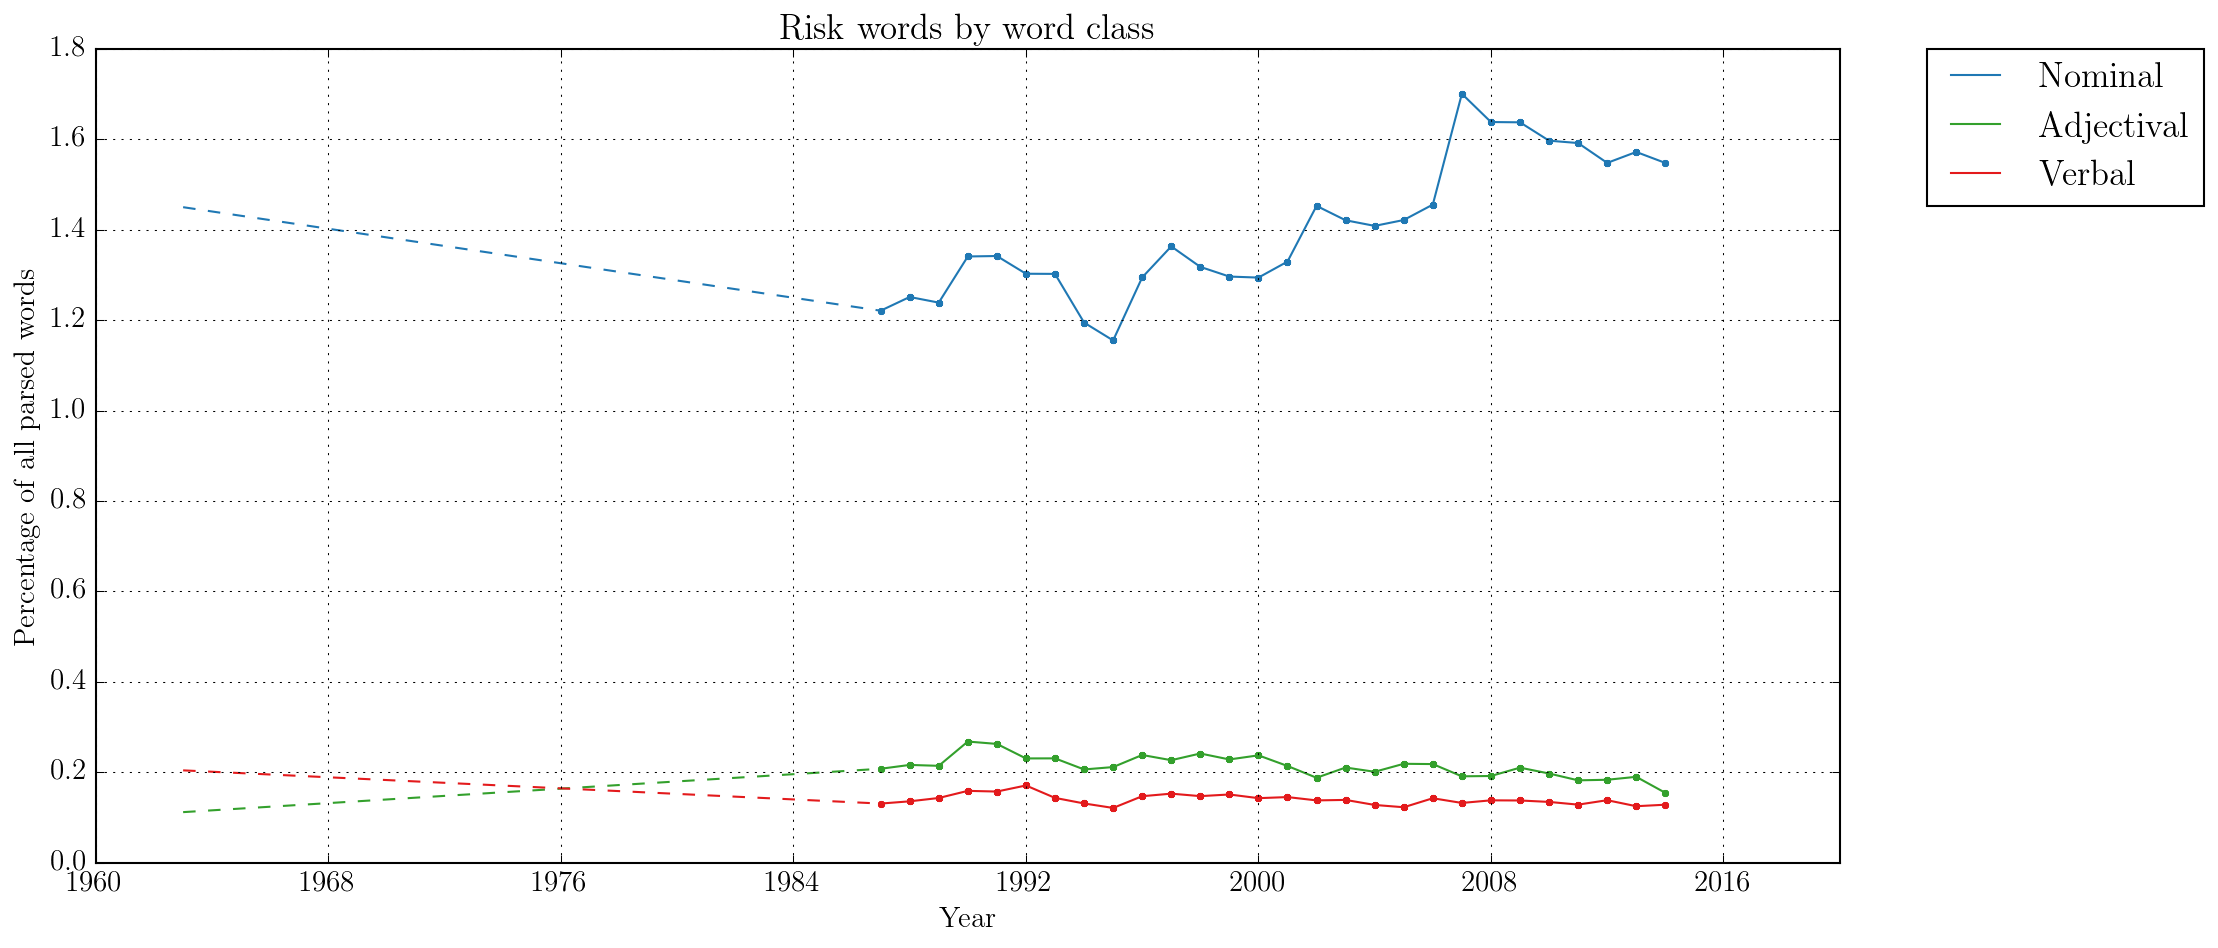
\includegraphics[width=0.75\textwidth]{../images/risk_words_by_word_class}}
%\caption{Risk words by word class (general corpus)}
%%\label{fig:comparison}
%\end{figure}



%\begin{figure}[htb!]
%\centering
%\addvbuffer[12pt 0pt]{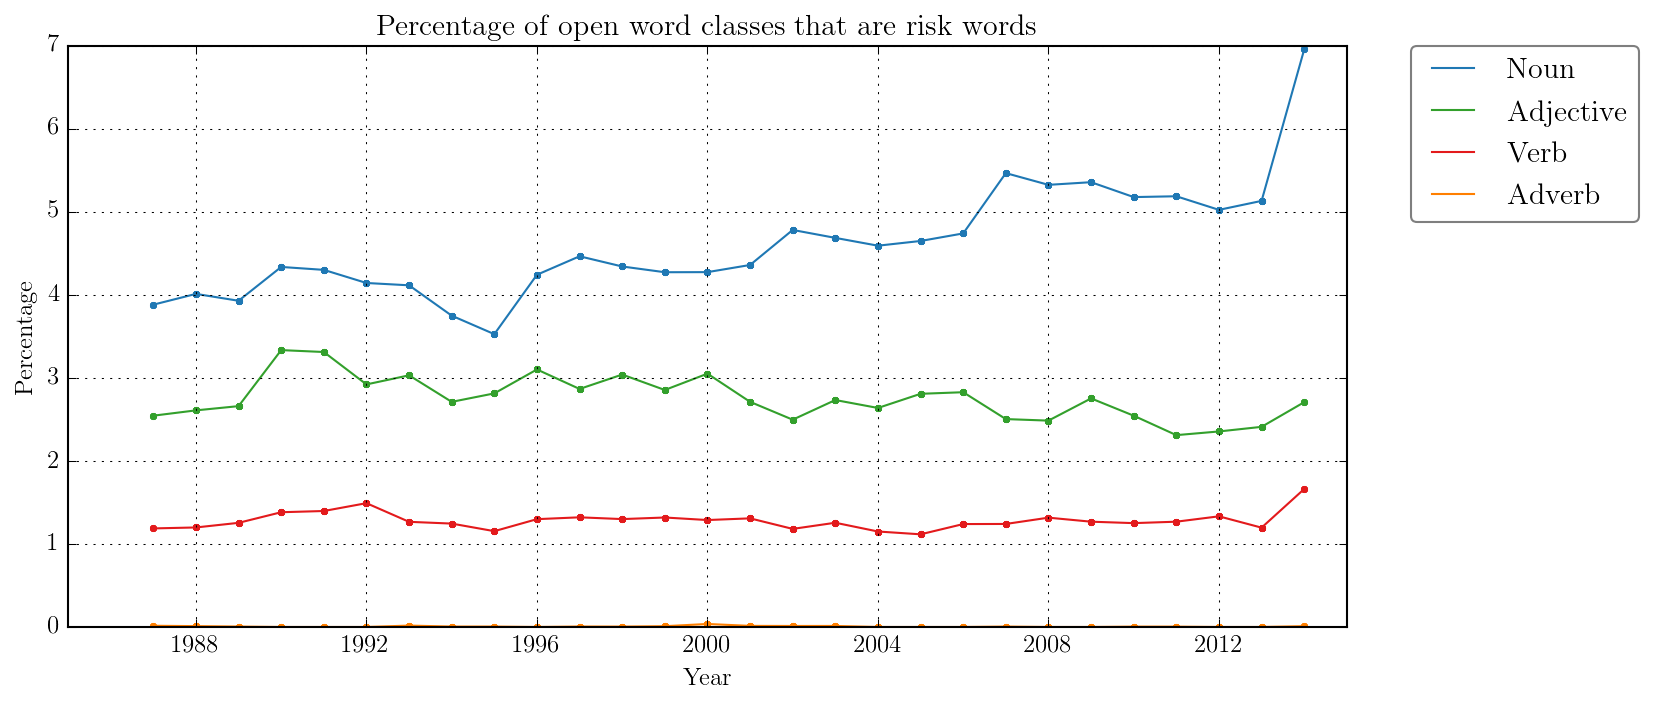
\includegraphics[width=0.75\textwidth]{../images/perc_open}}
%\caption{Percentage of open word classes that are risk words (general corpus)}
%%\label{fig:comparison}
%\end{figure}

As discussed earlier, nominal risks are often synonymous with negative outcomes, while verbal risks typically denote the entire process (an agent making the process occur, the change for negative or positive outcomes, etc.). Accordingly, trends toward nominalisation can be seen as evidence for the argument that risk more and more resembles only the negative components of the risk frame. 

Formal word class categories are not necessarily reliable means of determining which kind of risk semantic is being instantiated, however. Risk is nominal in `risk management', but is serving a modifier function. Risk is also nominal in 'to take a risk', but is really a part of the process, as in `to take a break' or `to have a shower'. Accordingly, we used Stanford CoreNLP's dependency parser to categorise risk words by experiential function, rather than grammatical form.

\begin{figure}[htb!]
\centering
\addvbuffer[12pt 0pt]{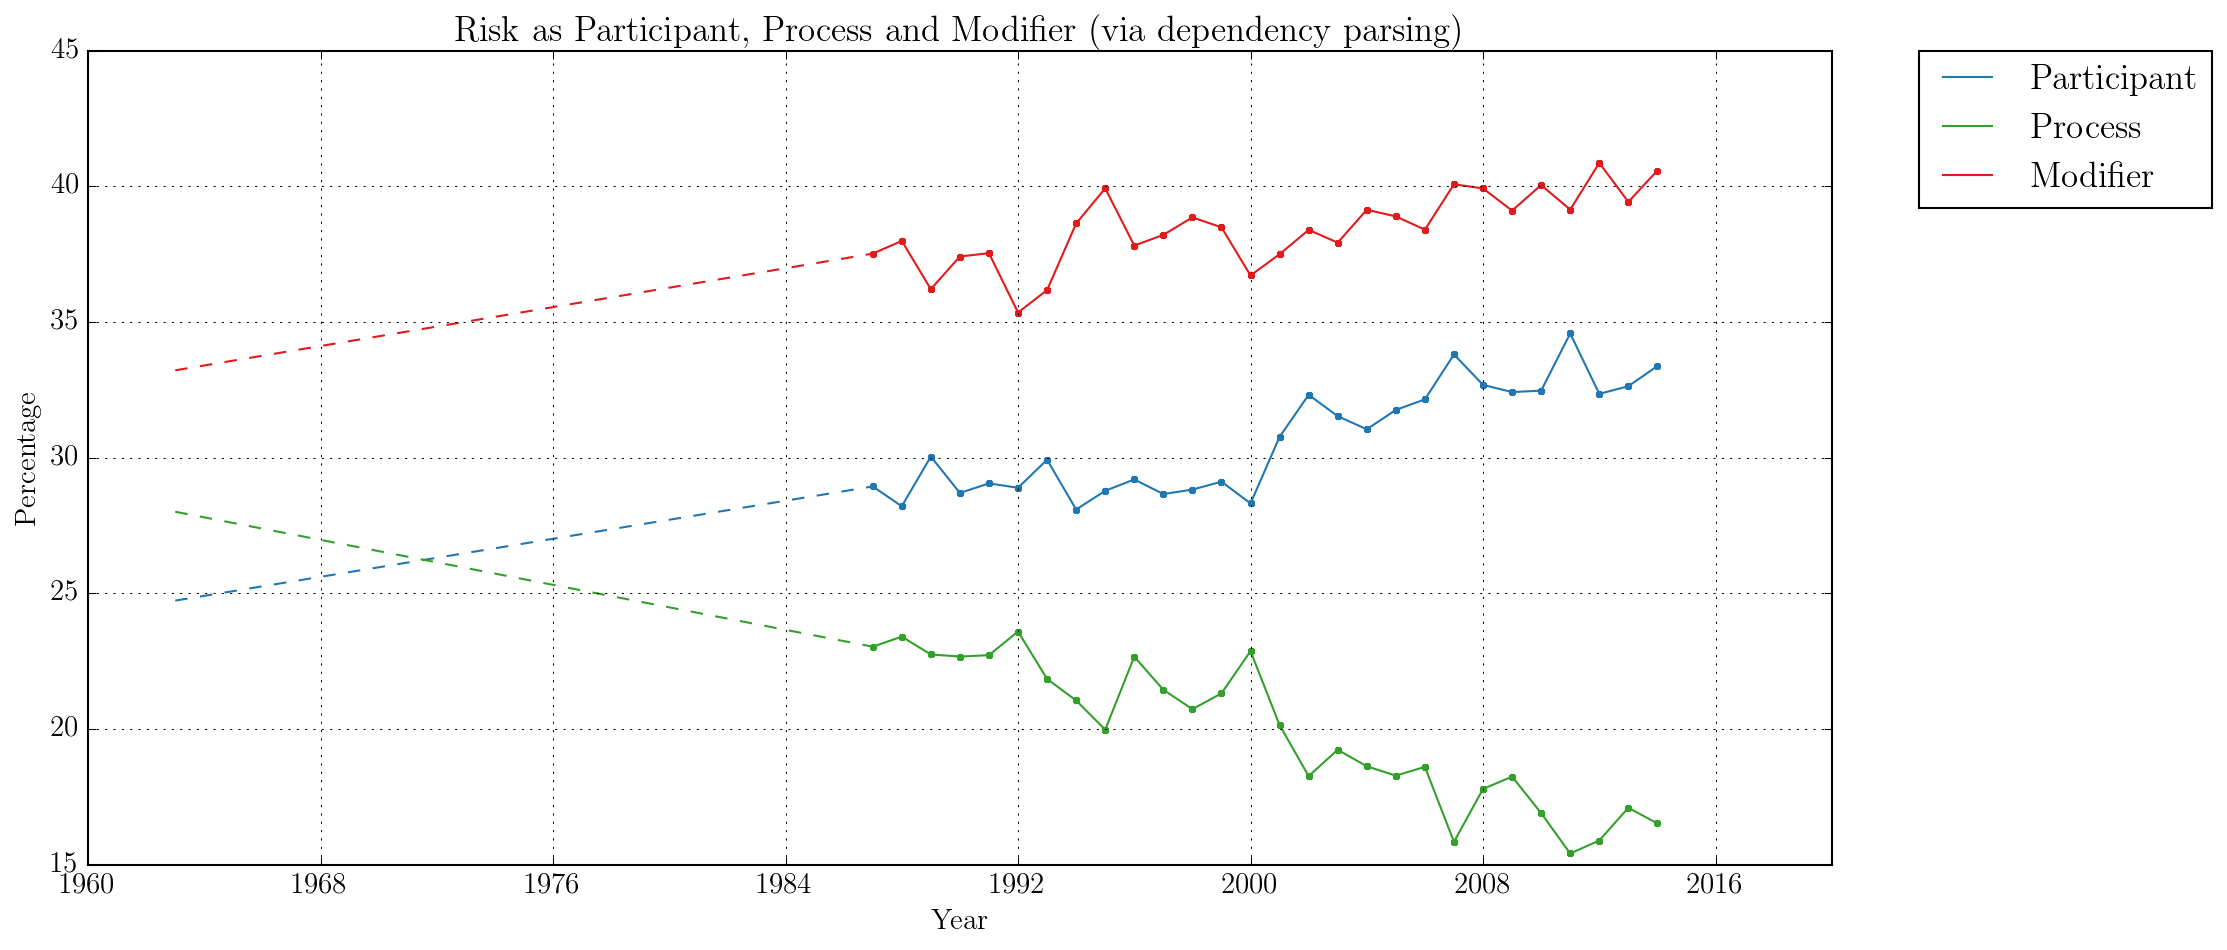
\includegraphics[width=0.75\textwidth]{../images/risk-as-participant-process-and-modifier-via-dependency-parsing}}
\caption{Risk as Participant, Process and Modifier (general corpus)}
%\label{fig:comparison}
\end{figure}

We find here a more accurate picture of the increasing synonymy of risk and negative outcomes, the shift away from the standard risk frame, and finally, a greater implicitness of risk. In SFL, the process is the central part of experiential meaning. The process and participants coupled together form the nucleus of the clause---they are what is effectively being discussed. Modifiers and circumstances, on the other hand, provide ancillary information, describing these participants, or the manner in which the process occurred. Shifts toward modifier forms thus suggest an increased implicitness of risk within the texts, where risk permeates discussion of an ever-growing set of domains, but less and less forms the propositional nub of what is being focally represented in the discourse.

\subsection{Shifts within risk words as participants, processes and modifiers}

To understand more precisely how risk discourse is changing, we can subdivide the experiential roles of participant, process and modifier.

\begin{figure}[htb!]
\centering
\addvbuffer[12pt 0pt]{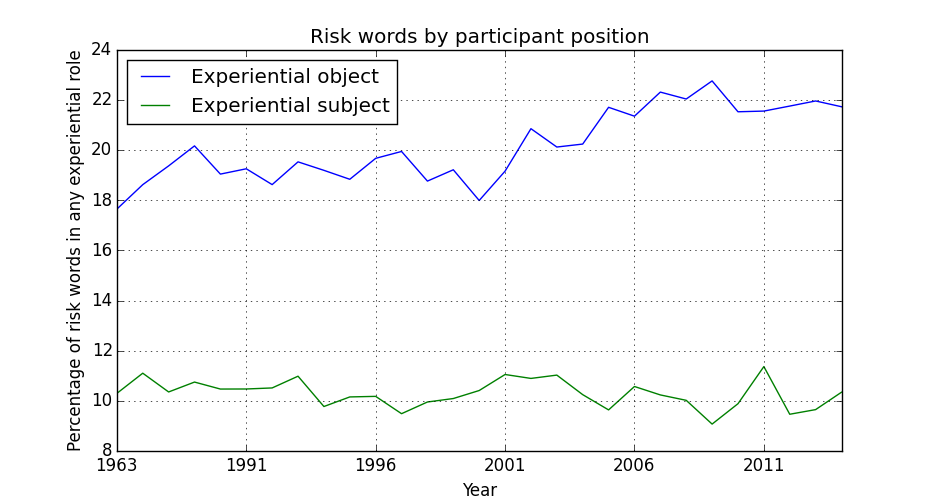
\includegraphics[width=0.75\textwidth]{../images/risk_as_exp_subj_and_obj}}
\caption{Risk as experiential subject\slash object (general corpus)}
%\label{fig:comparison}
\end{figure}

First, we can divide participants into those that occur as experiential subjects and experiential objects, with experiential subjects being more likely to be active agents, and more focal in the discourse. Consider the examples below (from 2010), with risk as experiential subject in Example 1 and experiential object in Example 2:

\begin{enumerate} [before=\color{black}\ttfamily] \setlength\itemsep{0em} \small
\item This risk, however, is minimal when compared to oil coating and ingestion.
\item Earlier studies found that running shoes could increase the risk for plantar fasciitis and ankle sprains.
\end{enumerate}

Given the steady rise in risk as an experiential object, it is reasonable to suggest that not only is risk increasingly synonymous with negative outcomes, but that it is also more implicit in meanings made about the world.

\subsection{From calculated to possibilistic risk}

We can also look at the kinds of adjectives modifying risk-as-participants in order to better understand the ways in which risks are judged or appraised in the NYT. As Max Weber has stated, rationalisation as a core characteristic of the modernisation process goes along with the belief that things should be rationally managed. Exactly this modern dream has been set under pressure in Late Modernity. As Beck has emphasised the modern techniques such as insurance would fail when dealing with new mega risks. Unexpected side-effects, high complexity and contradictory knowledge might create an unexpected feeling of being exposed to all kinds of risks without the ability to calculate and control them. It might be difficult to pin such a complex shift down easily. With this conceptualisation in mind, we examined the modifiers of risk used in the volumes of the NYT. Very dominant was the expression `high risk' with a clear peak during the H5N1 Asian Flu outbreak. It is interesting that we could found a clear trend in the last 25 years away from using risk in the context of the calculability of risk towards a general potentiality of risk.

\begin{figure}[htb!]
\centering
\addvbuffer[12pt 0pt]{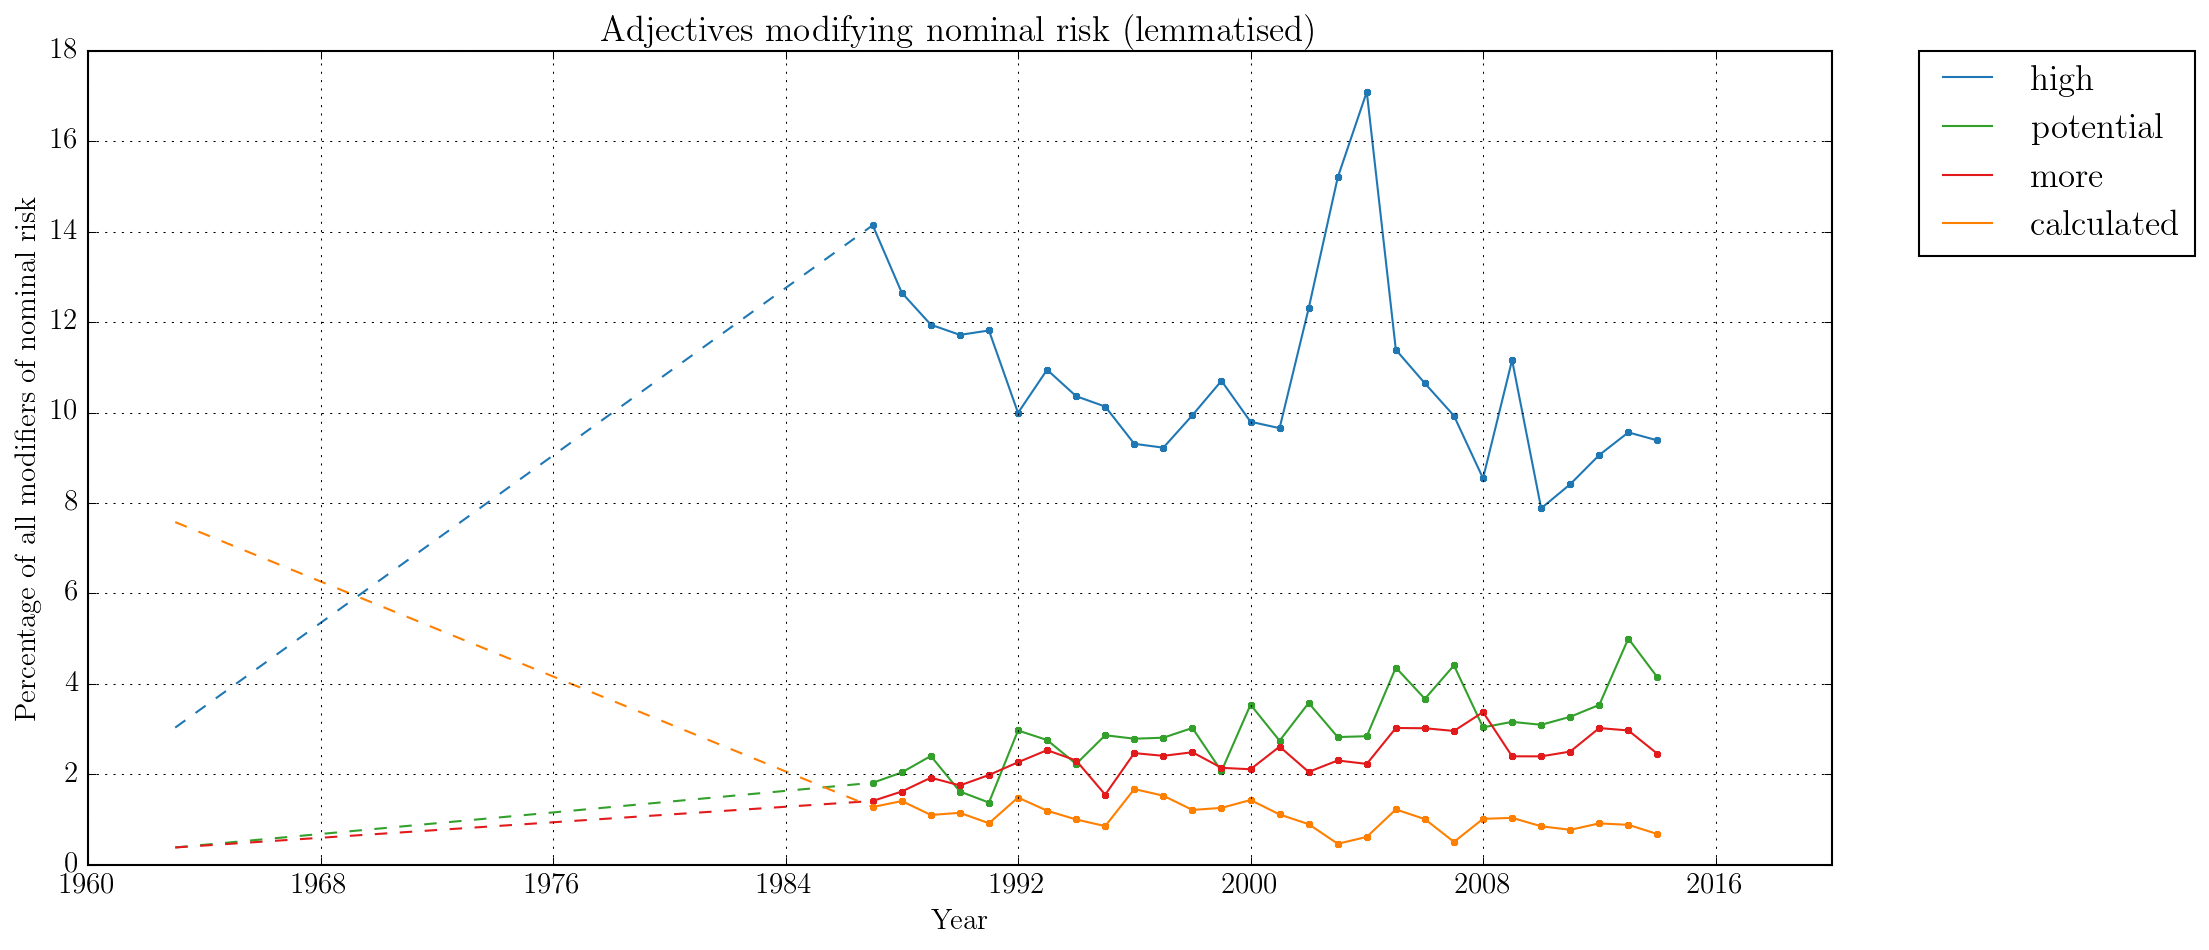
\includegraphics[width=0.75\textwidth]{../images/adjectives_modifying_nominal_risk_(lemmatised)}}
\caption{Adjectives modifying nominal risk (general corpus)}
%\label{fig:comparison}
\end{figure}

\subsection{Decreasing agency in risk processes (technocratic risk talk)}

Subdividing risk processes (Figure \ref{fig:pcs}), we can see that the `base' risk-process is declining steadily in frequency, with newer risk processes such as put at risk and pose risk overtaking running risk in frequency. Like the trend toward risk-as-participant, the changing climate of risk-as-process points to movement away from the standard risk frame. 

\begin{figure}[htb!]
\centering
\addvbuffer[12pt 0pt]{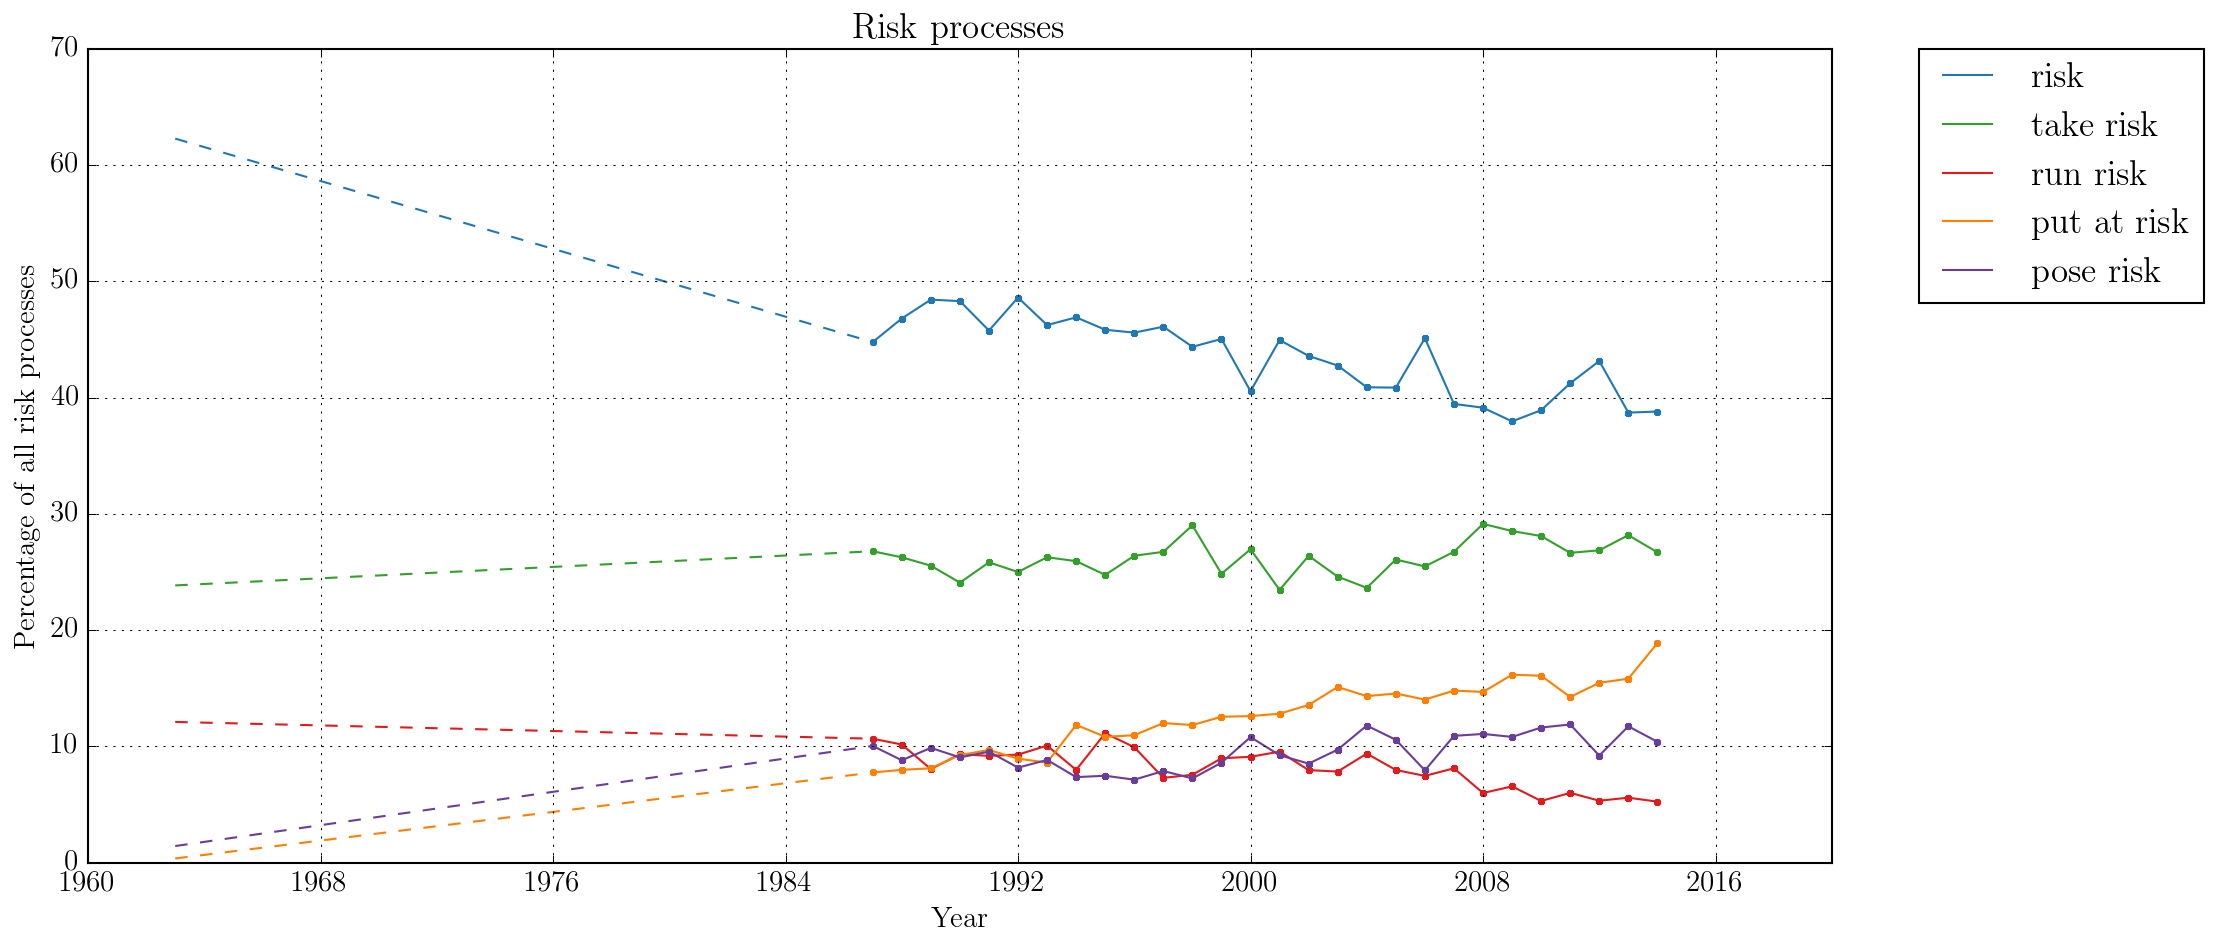
\includegraphics[width=0.75\textwidth]{../images/risk_processes}}
\caption{Risk processes (general corpus)}
\label{fig:pcs}
\end{figure}

While risking, taking risks and running risks all conform more or less to the semantic frames mapped out by Fillmore \& Atkins (1992), with a risker, and positive and negative outcomes, this is not the case with posing and putting at risk. In neither of these constructions does the actor take the role of the risker. In the pose risk construction, the risker here is optionally encoded in a circumstance beginning with the preposition `to'. From 2006:
%
\begin{enumerate} [before=\color{black}\ttfamily] \setlength\itemsep{0em} \small
\item The industry has also denied that electromagnetic emissions from overhead power lines pose any health risks.
\item But if the newer antidepressants posed a significant suicide risk, suicide attempts would probably rise, not fall, after treatment began, Dr. Simon said.
\item Those deemed by a judge to pose a greater risk to themselves or others are housed at the Bergen County Jail in Hackensack.
\item The ministry said the workers posed no risk to others and had the A (H5N2) virus, a milder strain than A (H5N1) which has killed more than 70 people.
\item Finance ministers from the world's richest countries and Russia said Saturday that `high and volatile' energy prices posed a risk to global economic growth that otherwise appeared solid.
\end{enumerate}
%
This same distinction is even clearer in \emph{put at risk}, whose actor tends to be an inanimate of abstract noun, and whose experiential object is generally a broad group of everyday people, such as women, children, or citizens. The following examples are from NYT articles on health topics from 2012:
%
\begin{enumerate} [before=\color{black}\ttfamily] \setlength\itemsep{0em} \small
\item Pharmacists also overlooked or approved cases in which medications were prescribed at questionable levels or in unsafe combinations that could put patients at risk of seizures, accidents or even death, according to the public health department.
\item It also cited studies showing that women with unintended pregnancies are more likely to be depressed and to smoke, drink and delay or skip prenatal care, potentially harming fetuses and putting babies at increased risk of being born prematurely and having low birth weight.
\item Last September, Qualitest Pharmaceuticals, a unit of Endo Pharmaceuticals, voluntarily recalled `multiple lots' of contraceptive pills -- also because of a `packaging error' that could put women at risk for pregnancy.
\item Representative Chris Smith, a New Jersey Republican and leader of the House anti-abortion forces, said the latest announcement demonstrated that the president `will use force, coercion and ruinous fines that put faith-based charities, hospitals and schools at risk of closure, harming millions of kids, as well as the poor, sick and disabled that they serve, in order to force obedience to Obama's will.'
\item The Japanese government's failure to warn citizens about radioactive danger put the entire city of Tokyo at health risk -- and the rest of us as well.
\end{enumerate}
%
These results support the hypothesis of degreasing agency in risk reporting.
%
\subsection{The institutionalisation of risk practices}

Risk-as-modifier is very common because they encompass a number of diverse sub-categories: risk may be (among other things) an adjectival modifier (a risky decision), an adverbial modifier (he riskily chose), a nominal modifier (risk management) or the head of a nominal group inside a prepositional phrase, serving the role of modifying the main verb of the clause (They were appalled by the risk). 

\begin{figure}[htb!]
\centering
\addvbuffer[12pt 0pt]{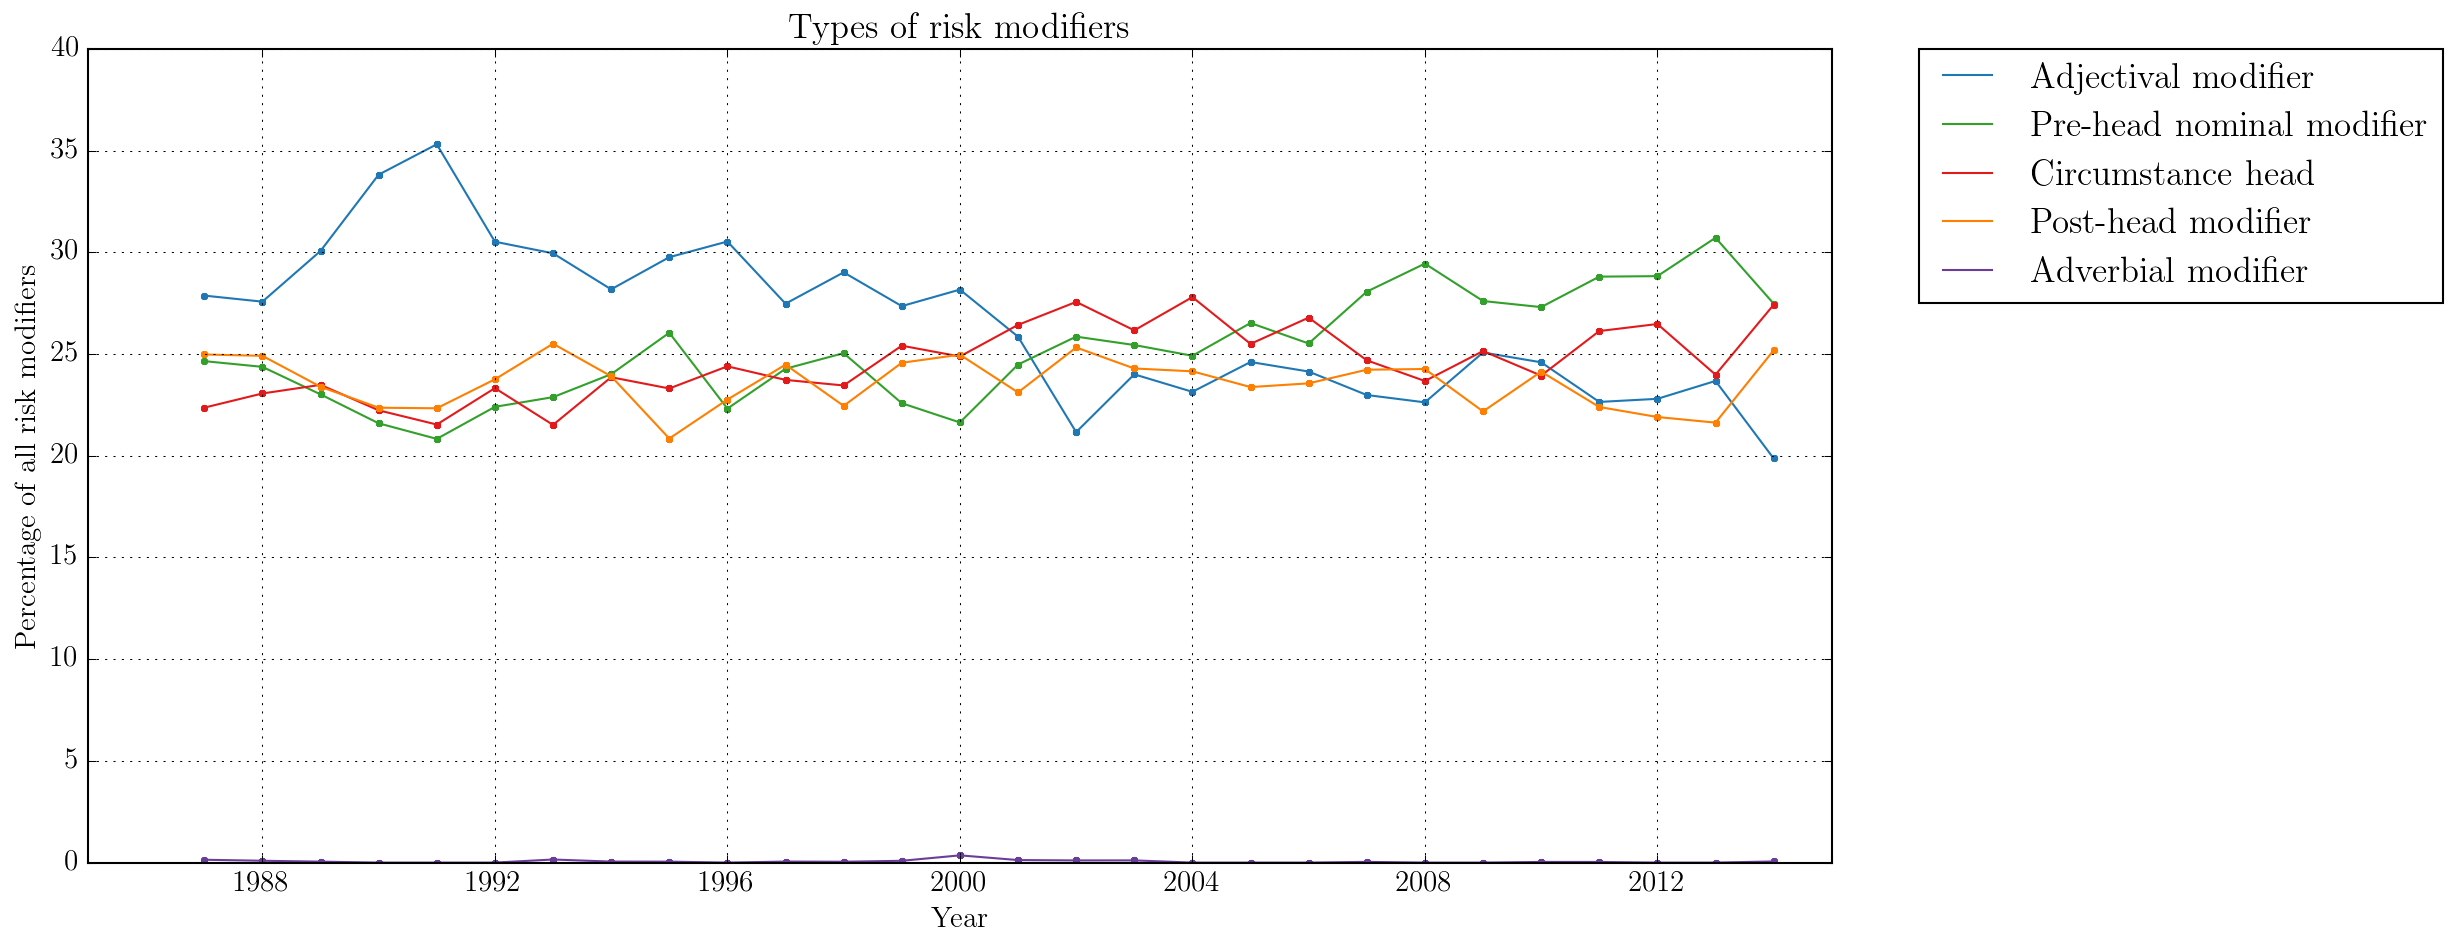
\includegraphics[width=0.75\textwidth]{../images/old-types-of-risk-modifiers}}
\caption{Types of risk modifiers (general corpus)}
%\label{fig:comparison}
\end{figure}

By charting these different forms, an interesting picture emerges: adjectival modifiers decline gradually in frequency, while nominal modifiers (examples from 2012 below) rise. 

\begin{enumerate} [before=\color{black}\ttfamily] \setlength\itemsep{0em} \small
\item `That's why more companies are turning to certified financial risk managers,' the ad continues.
\item Many clients asked Teresa Leigh, owner of Household Risk Management, a North Carolina-based advisory service for wealthy households, to explain just what all the headlines are about.
\item Rather than downsizing their lifestyles, `they're spending more money on protecting their homes,' said Paul M. Viollis Sr., the chief executive of Risk Control Strategies, a security advisory firm based in New York City, whose clients have an average net worth of more than \$100 million.
\item A recent survey by the Spectrem Group found that `while somewhat more moderate in risk tolerance than in 2009, investors remain more interested in protecting principal than growing their assets.'
\item Mr. Munson suggested a more enlightened view that looks at `risk budgeting,' or gauging how much risk you can take, and design a portfolio that tracks your tolerance -- or intolerance -- for stock market exposure.
\end{enumerate}


Foremost, this supports the idea that institutions increasingly devote special attention to risk. Importantly, adjectives attach to nouns very freely, but nominal modification of nouns requires some kind of codification within the culture: a novel situation may be described as a risky one, but risk arbitrage is an activity created explicitly to handle the phenomenon of risk. As such, nominal modifiers are an important signifier that risk has taken on a more and more central and tangible role within institutions.

\subsection{Risk takers and risk bearers}

We have seen that expressions of active risk taking are in decrease while more `technocratic' expressions (to pose\slash put at risk) express that less agency expressions are on the rise. This is surprising, considering hypothesis of governmentality or individualisation theorists that institutions would increasingly expect that individuals manage risks themselves. If this is expected, we would at least expect that terms such as person, man and woman are addressed in risk reporting even when they are not in power but exposed to risk. Individualisation processes would then be reflected in the news coverage of the NYT in reporting the opposite of what is desirable, the exposure to risk of the vulnerable.

Grammatical annotation can be used to look for the subjects of risk processes whose subject is the agent behind the risk (to risk, to run risk, to take risk, to put at risk). By focussing on the most common grammatical riskers, we can see that person\slash people, companies, banks, states, investors, governments, man\slash men and leaders are leading the riskers overall in the NYT. The list thus contains both powerful institutions and terms often used for everyday people. 

\begin{figure}[htb!]
\centering
\addvbuffer[12pt 0pt]{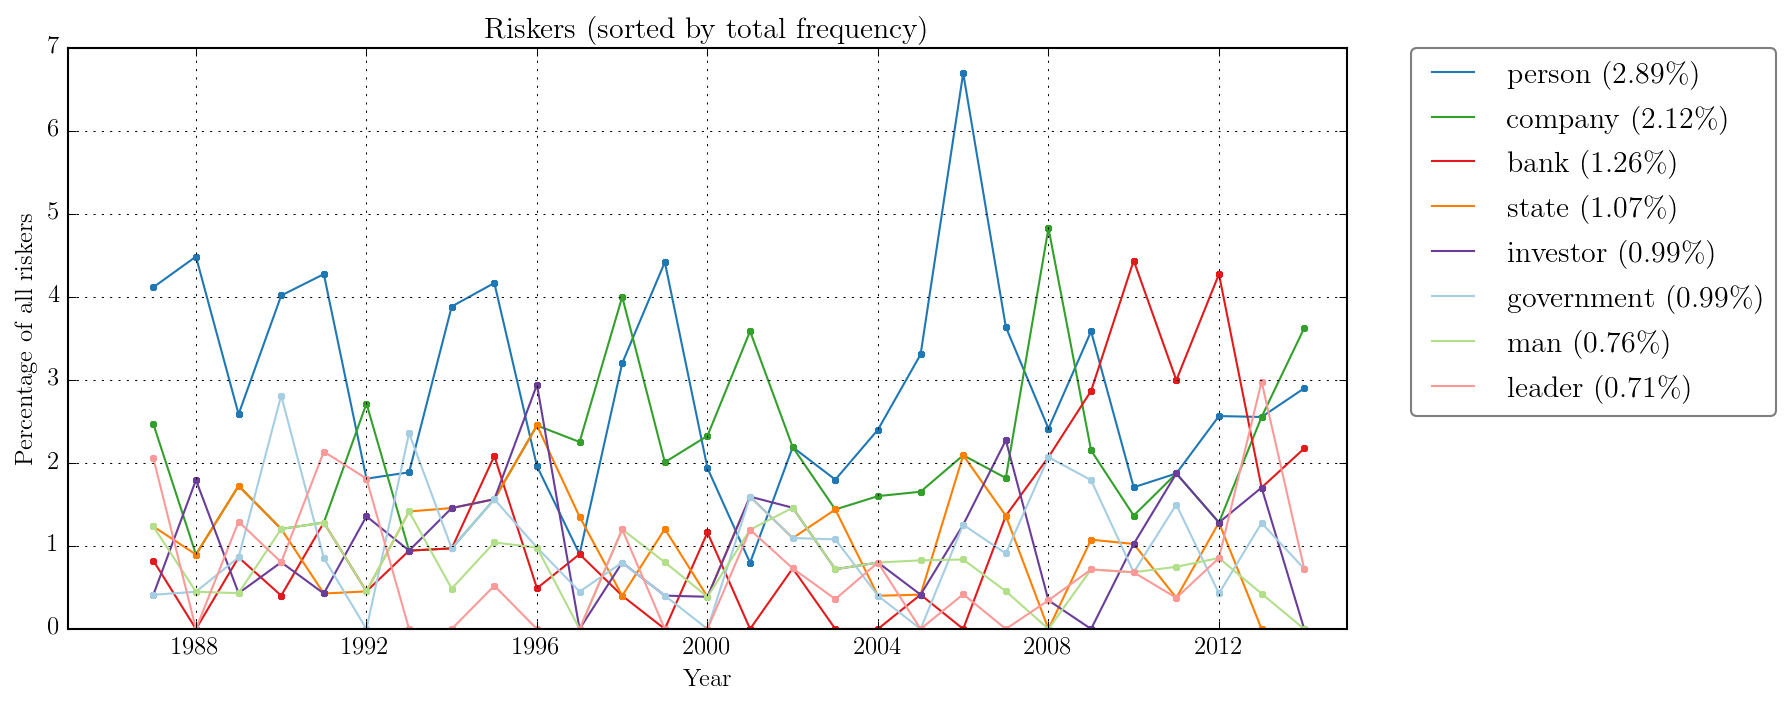
\includegraphics[width=0.75\textwidth]{../images/riskers-sorted-by-total-frequency}}
\caption{Riskers (general corpus)}
%\label{fig:comparison}
\end{figure}

To examine the role of risker more closely, we created a list of all heads of nominal groups in the corpus, and determined the percentage of the time that noun occurs as the actor in a risk process. This involves determining a sensible threshold for the minimum number of total occurrences, lest the top results be simply words that only appeared once, as a risker, in the dataset. Thus, words appearing fewer than 750 times in the corpus were excluded.

\begin{figure}[htb!]
\centering
\addvbuffer[12pt 0pt]{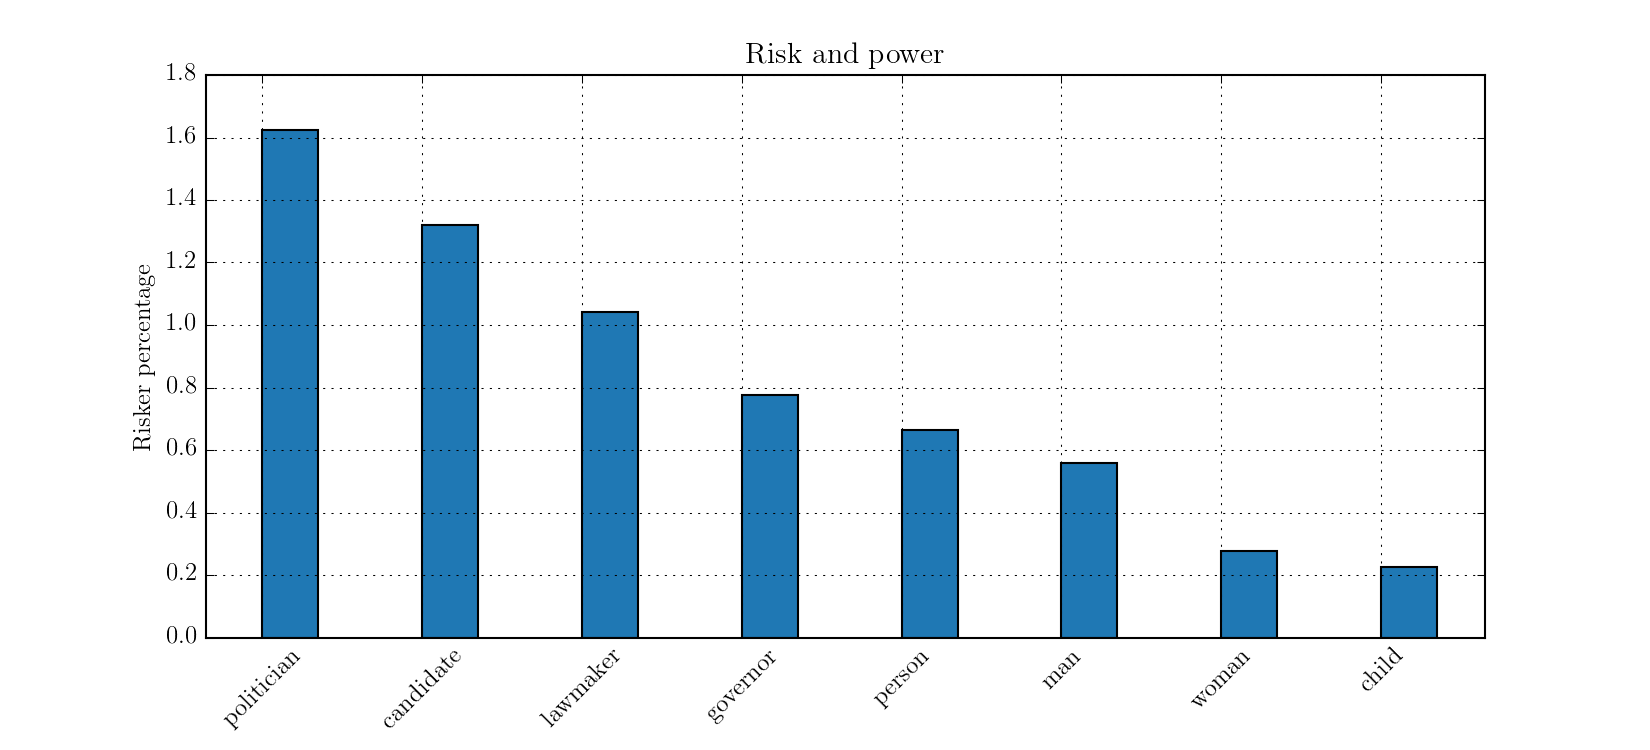
\includegraphics[width=0.75\textwidth]{../images/risk-and-power}}
\caption{Percentage of common participants that are in the role of risker (general corpus)}
%\label{fig:comparison}
\end{figure}

The division between powerful people in government and law, compared to everyday terms for average people, is startling:

\begin{multicols}{2}
\begin{enumerate} [before=\color{black}\ttfamily] \setlength\itemsep{0em} \small
\item Today, George W. Bush, with his dauphin's presumption that the Presidency is his for the taking and his cocky refusal to depart from his canned stump speech, may risk repeating Dewey's error and give his opponents the sentimental underdog's advantage.
\item After months of giving President Fox the cold shoulder, Mr. Bush's action on immigration may foretell an end to the tensions, particularly since Mr. Bush is taking a political risk by angering anti-immigration Republicans.
\item By raising the question of his role in the Iran arms-for-hostages deal, even to decry those questions as part of a `Democrat-run' witchhunt, Mr. Bush risked appearing defensive and risked prolonging news coverage of a six-year-old scandal that has already eaten up one of his last four days of campaigning.
\item Longtime Washington observers question if Mr. Obama would risk a battle over his secretary of state
\item Ignoring the fact that it's her beloved Tea Party dragging the country to ruin, Palin suggested on Facebook that if the country defaults on its debt, Obama is risking impeachment. 
\end{enumerate}

\begin{enumerate} [before=\color{black}\ttfamily] \setlength\itemsep{0em} \small
\item Perfectly normal men and women were risking prison by making a pass at someone.
\item `Some people will clearly risk death to reach Europe,' said Israel D\'{i}az Arag\'{o}n, who captains one of the boats of Spain's maritime rescue services.
\item Even those women who become cam models of their own free will take on serious risks associated with sex work
\item People who were lactose intolerant could have risked losing water from diarrhea, Dr. Tishkoff said.
\item The humiliating result, six workers said in separate interviews, was that men were sometimes forced to urinate in their pants or risk heat exhaustion.
\end{enumerate}
\end{multicols}
%
Thus, not only are everyday people increasingly lacking agency in the risk process. Contextualised instances of different kinds of riskers reveals that the kinds of things that are risked are less abstract, and often with little balance between the possible positive and negative outcomes.

We will see later on when examining health articles that women, person, man, child, consumer and baby all occur regularly as participants but as we have seen here with less agency when powerful institutional actors while it is the banks, companies, firms and agencies which are increasingly reported as riskers while person, man and woman are on an upwards slope (compare Zinn \& McDonald 2015).

\subsection{The Risk Semantic in Health Discourses}

Findings from an earlier investigation have shown that health plays a larger role in risk discourse in 2000 than it did in 1900. We were interested in both whether we can confirm the significance of health through linguistic analysis, and whether a richer picture of the relationship between risk and health could be provided. Given the attention paid by Beck to the status of science and research in reflexive modernity, a particular focus was on the ways in which risk, health and research co-occur. 

\begin{figure}[htb!]
\centering
\addvbuffer[12pt 0pt]{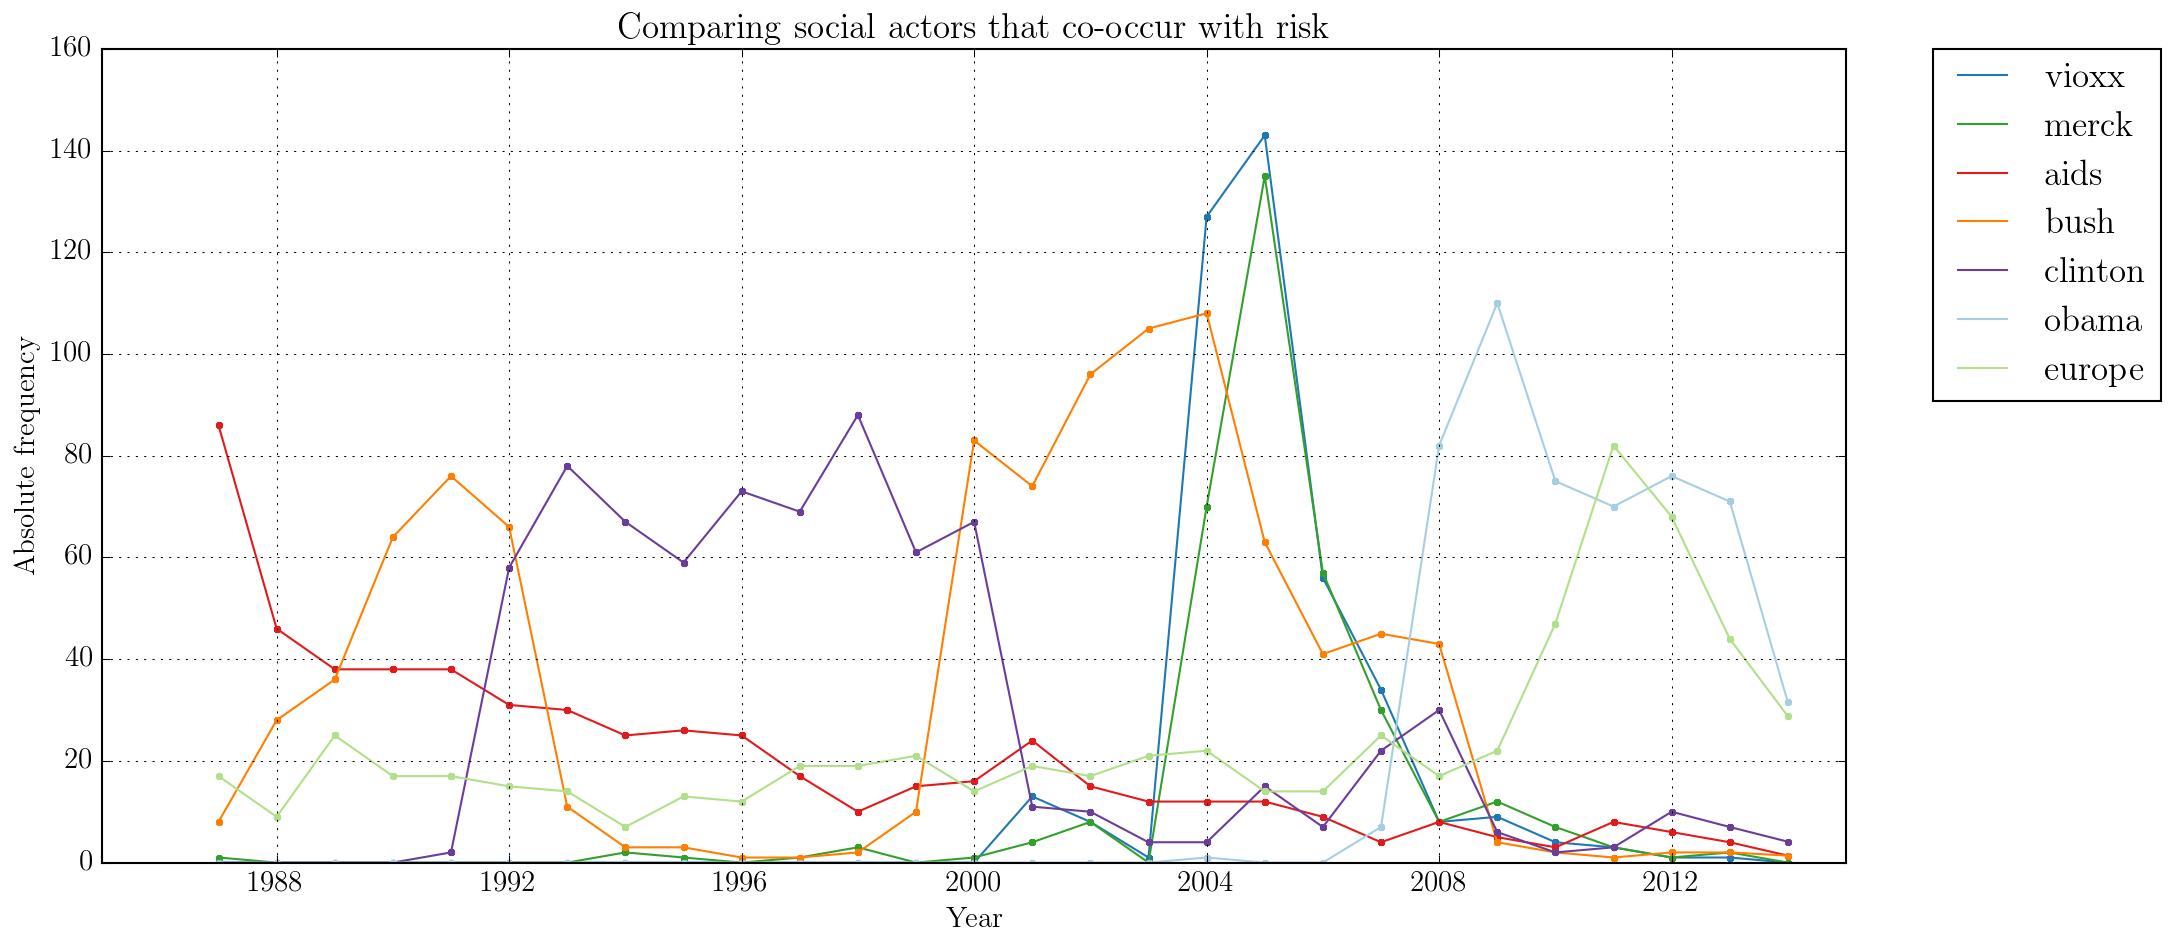
\includegraphics[width=0.75\textwidth]{../images/comparing_social_actors_that_co-occur_with_risk}}
\caption{Comparing social actors that co-occur with risk}
%\label{fig:comparison}
\end{figure}

The salience of health topics is clear: in their most prominent years, AIDS, Vioxx and Merck comprise over 1.6 per cent of all proper nouns that co-occur with a risk word. This is higher than Clinton, Bush or Obama at their peaks, as well as Soviet Union in 1987 or Europe during the Eurozone crisis in 2011.

\begin{table}
\footnotesize
\begin{tabular}{rcl}
of a crucial clinical trial of the painkiller      &     Vioxx    &   to play down its heart risks \\

he questioned her about the details of data about   &  Vioxx's    & risks of causing heart attacks \\

popular painkillers like Pfizer's Celebrex or    &  Merck's     &    Vioxx increased the risk of  \\heart attacks
\end{tabular}
\end{table}
\begin{table}
\footnotesize
\begin{tabular}{rcl}
Yet the United States and           &        Europe    &      face the risk that their problems will feed on \\
There is a risk over time that democracy will lead &   Europe  &    to splinter \\
In addition,  &   Europe  &    is ailing, there is a risk that oil prices will \\
\end{tabular}
\end{table}

Further evidence for the salience of health topics when compared to others was found by searching for nominal modification of risk-as-participant (e.g. the cancer risk\slash the risk of cancer) to uncover more explicit marking of the negative outcomes in the corpus of all risk tokens.

\begin{figure}[htb!]
\centering
\addvbuffer[12pt 0pt]{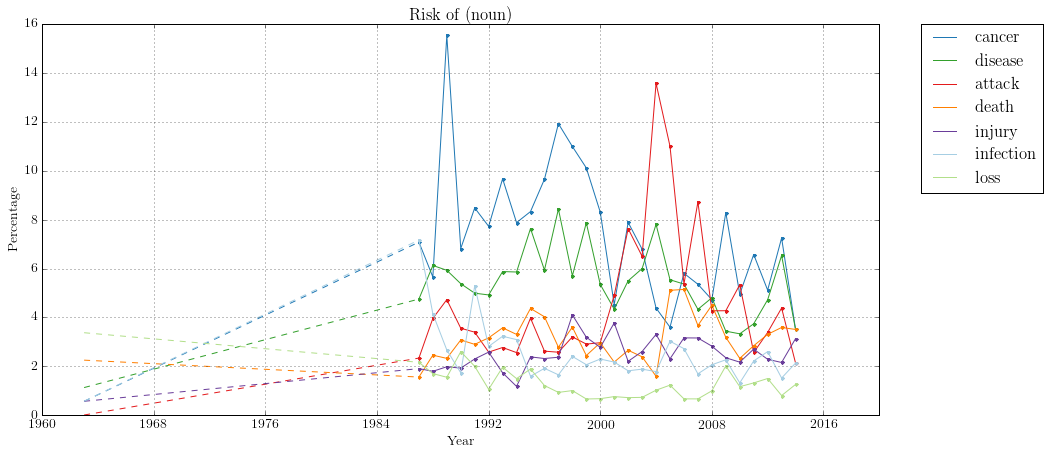
\includegraphics[width=0.75\textwidth]{../images/riskofnoun}}
\caption{Risk of (noun) (general corpus)}
%\label{fig:comparison}
\end{figure}

Concordancing these examples revealed the sharp rise in 'risk of attack' has very little to do with war or terrorism, but instead, is almost always referring to the increased risk of heart attack discovered in those who take Vioxx. From 2004, for example: 

\begin{enumerate} [before=\color{black}\ttfamily] \setlength\itemsep{0em} \small
\item It reported that both drugs appeared to increase the risk of heart attack and stroke, but that the danger from Vioxx appeared higher.
\item In an April 2004 study in the journal Circulation, researchers from Harvard Medical School found that Vioxx raised the risk of heart attacks relative to Celebrex; two months later, several of the same researchers reported in another journal that Vioxx increased the risk of hypertension.
\end{enumerate}

\subsection{The shift towards individualism in health discourse}

By locating all participants in the health subcorpus, and sorting by those on increasing and decreasing paths, we can see broad shifts in the climate of health risks that are responsive to both events and broader social change: heightened discussion of health insurance in the USA in the early 1990s is related to the Clinton Healthcare Plan (1993), for example. That said, despite the more recent U.S. healthcare reform (beginning with the Affordable Care Act of 2009), insurance-related participants do not re-emerge in the later samples of the corpus, potentially indicating broader shifts in health\slash risk discourse that require further attention.

\begin{figure}[htb!]
\centering
\addvbuffer[12pt 0pt]{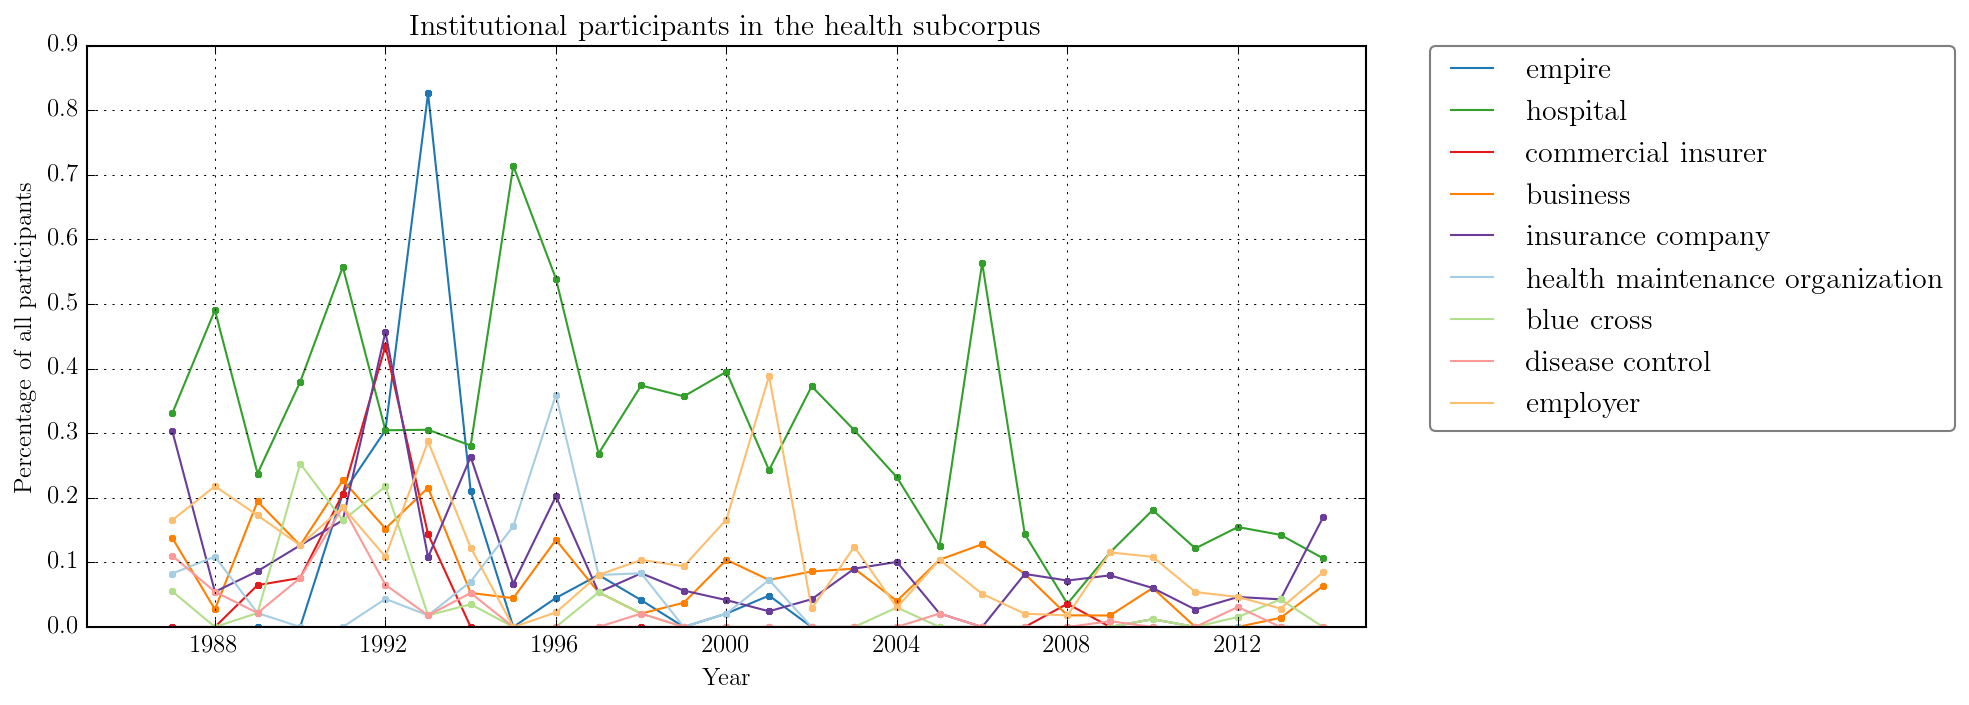
\includegraphics[width=0.75\textwidth]{../images/institutional-participants-in-the-health-subcorpus}}
\caption{Institutional participants (health subcorpus)}
%\label{fig:comparison}
\end{figure}


\begin{enumerate} [before=\color{black}\ttfamily] \setlength\itemsep{0em} \small
\item The bill, which became law on April 1, forces commercial insurance companies to accept any small-business applicant and to charge uniform rates, regardless of risk of illness, as Empire does.
\item Empire used the false data in its successful lobbying campaign last year for changes in state insurance law intended to force competitors to accept some high-risk customers.
\end{enumerate}

In contrast, most of the everyday participants in the health subcorpus are on the rise. That means that the trends in the health subcorpus might in some respects differ from the overall trend. Risk is increasingly communicated with vulnerable social groups such as women, children and babies but also with persons more generally, men and consumers.

\begin{figure}[htb!]
\centering
\addvbuffer[12pt 0pt]{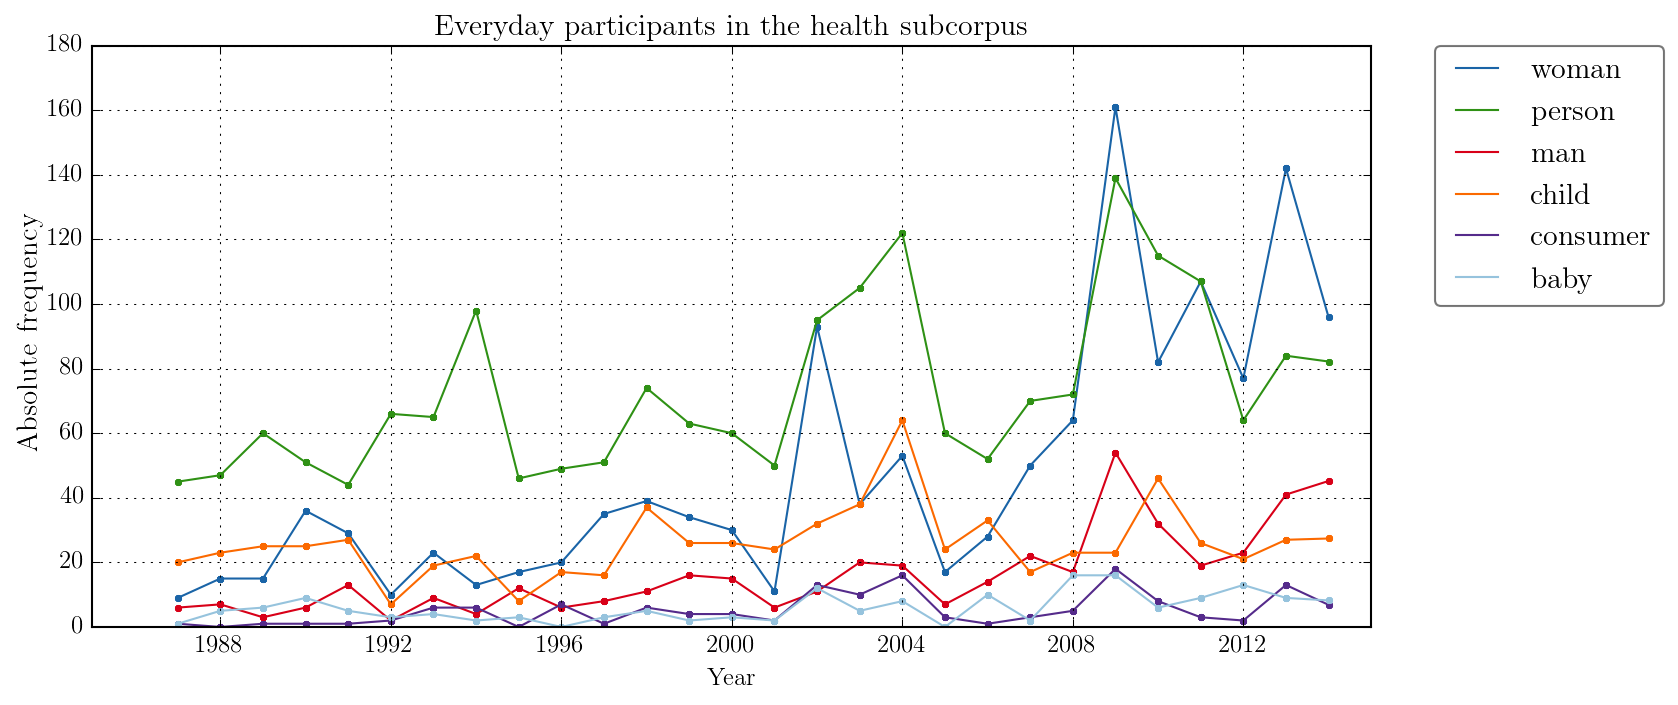
\includegraphics[width=0.75\textwidth]{../images/everyday-participants-in-the-health-subcorpus}}
\caption{Everyday participants (health subcorpus)}
%\label{fig:comparison}
\end{figure}

Our analysis of n-grams (recurring combination of two-word combinations from open word classes) showed that a number of civilisation illnesses and related health issues such as heart disease, heart attack, prostate cancer, ovarian cancer, lung cancer, blood clots and mental health, giving evidence of the prominence of cancer, heart disease and mental health issues in media coverage of recent debates. At the same time debates about health insurance, health plan, commercial insurer and insurance company decrease, indicating (as with the analysis of participants in the health corpus) that these debates they exist no longer reference to risk as a significant concept. The use of the risk semantic in the health sector is increasingly used in relation to everyday life people presented as vulnerable groups and decreasingly in the context of organisations. 

\begin{figure}[htb!]
\centering
\addvbuffer[12pt 0pt]{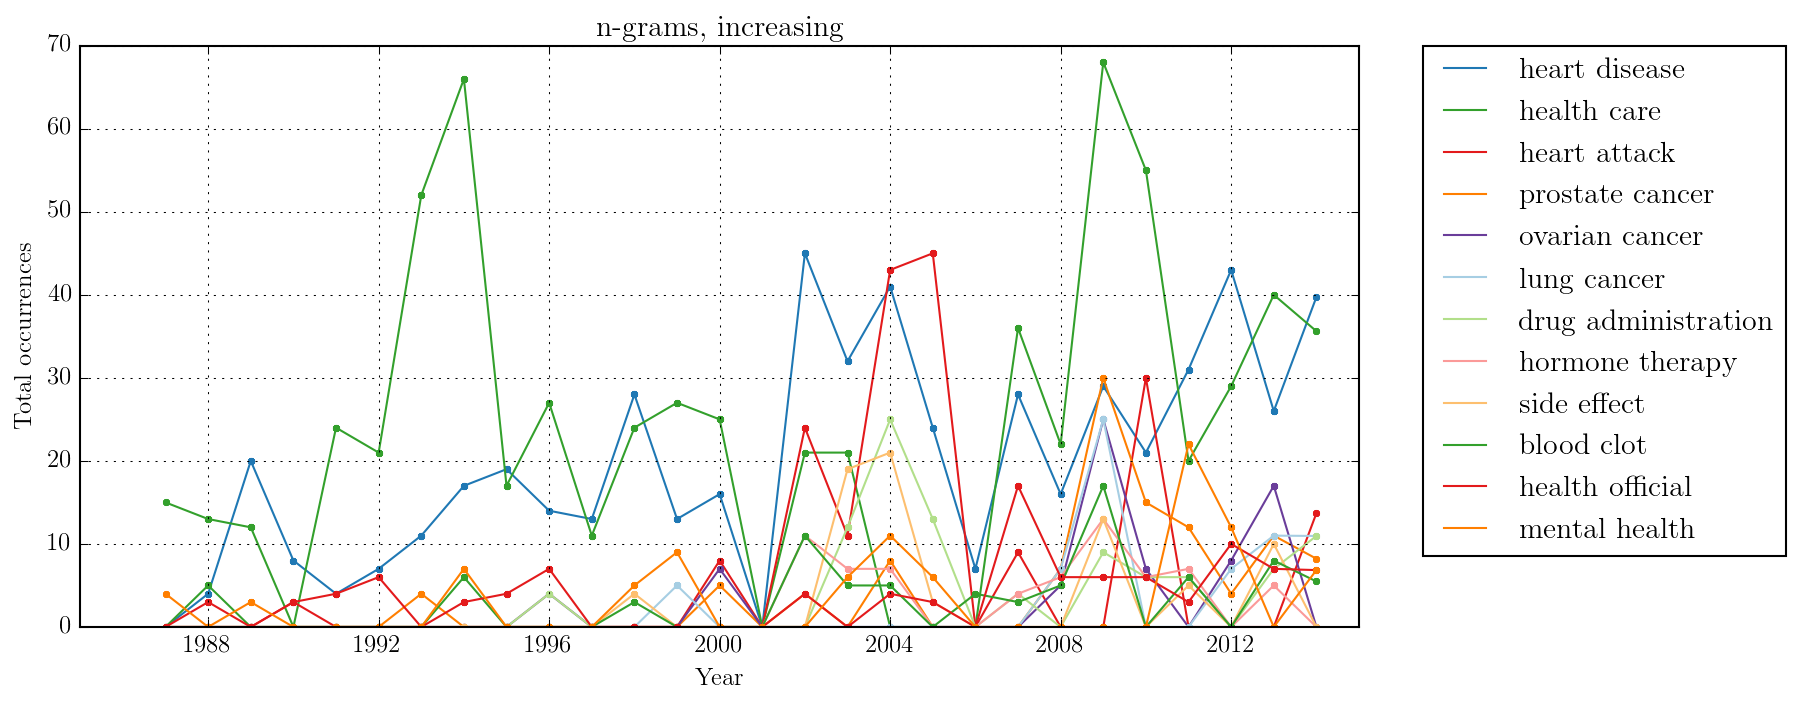
\includegraphics[width=0.75\textwidth]{../images/ngrams-increasing}}
\caption{n-grams, increasing (health subcorpus)}
%\label{fig:comparison}
\end{figure}


\begin{figure}[htb!]
\centering
\addvbuffer[12pt 0pt]{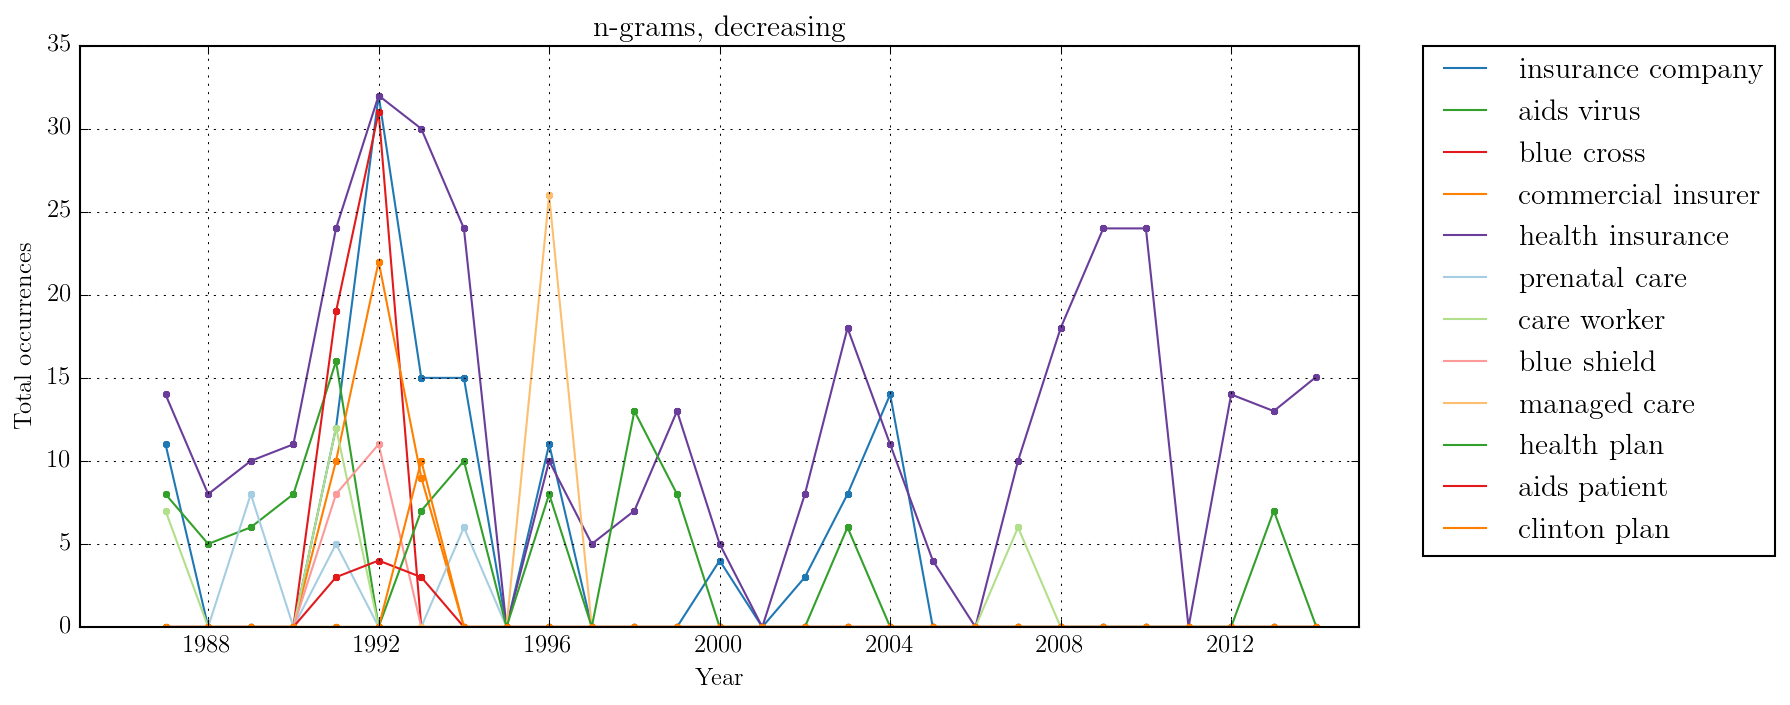
\includegraphics[width=0.75\textwidth]{../images/ngrams-decreasing}}
\caption{n-grams, decreasing (health subcorpus)}
%\label{fig:comparison}
\end{figure}


\subsection{Health discourse is driven by increasing reference to scientific expertise}

There is large support from different scholars that risk reporting is driven by journalism that refers to scientific experts and empirical evidence. While Mairal (2011) claimed that this is characteristic for a particular genre of journalism that developed in journalism during modernisation. Also, Beck's claim that the loss of scientific expertise does not lead to a decrease but increase of importance of scientific evidence supported the view that we should expect more reference to scientific expertise whether to research, scientific evidence or experts. Skolbekken's study on the risk epidemic in medical journals has shown that at least for scientific journals the increase in risk communication has manifested but the question remained to what extent this shift towards risk has also affected reporting in news media. 

\begin{figure}[htb!]
\centering
\addvbuffer[12pt 0pt]{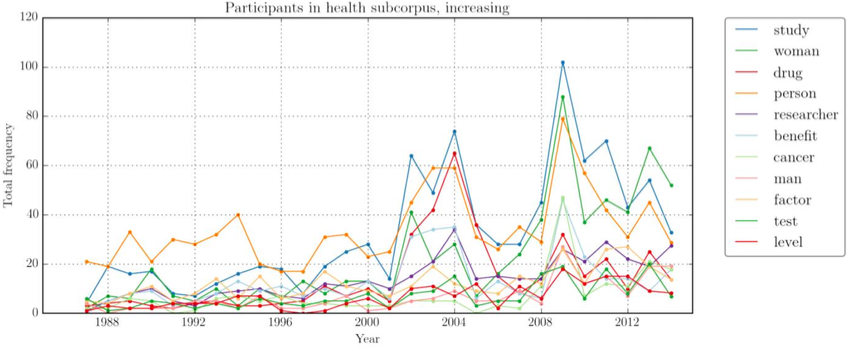
\includegraphics[width=0.75\textwidth]{../images/part_inc}}
\caption{Participants, increasing (health subcorpus)}
%\label{fig:comparison}
\end{figure}

Our analysis of participants in the health subcorpus supports the assumption that research-related participants in the discourses have increased over last decades. Of the top 11 increasing participants, two are explicitly associated with science and research (study, researcher), while other terms can be concordanced to reveal strong associations with this topic (factor, test, level).

In summary of the overall trends in the health subcorpus we have grouped the different infectious diseases (\emph{aids, aids virus, aids patient, transmission, flu, influenza}), everyday people (\emph{person, man, woman, child, baby, consumer}), institutions (\emph{empire, hospital, commercial, business, insurance company, HMO\slash health maintenance organisation, blue cross, disease control, employer, insurer, health insurance association, insurance industry, office}) and non-infectious diseases (\emph{breast cancer, cancer, heart disease, diabetes, heart attack, prostate cancer, stroke, ovarian cancer, obesity}) as well as science and research (\emph{study, researcher, finding, new study, author, university, expert}).

\begin{figure}[htb!]
\centering
\addvbuffer[12pt 0pt]{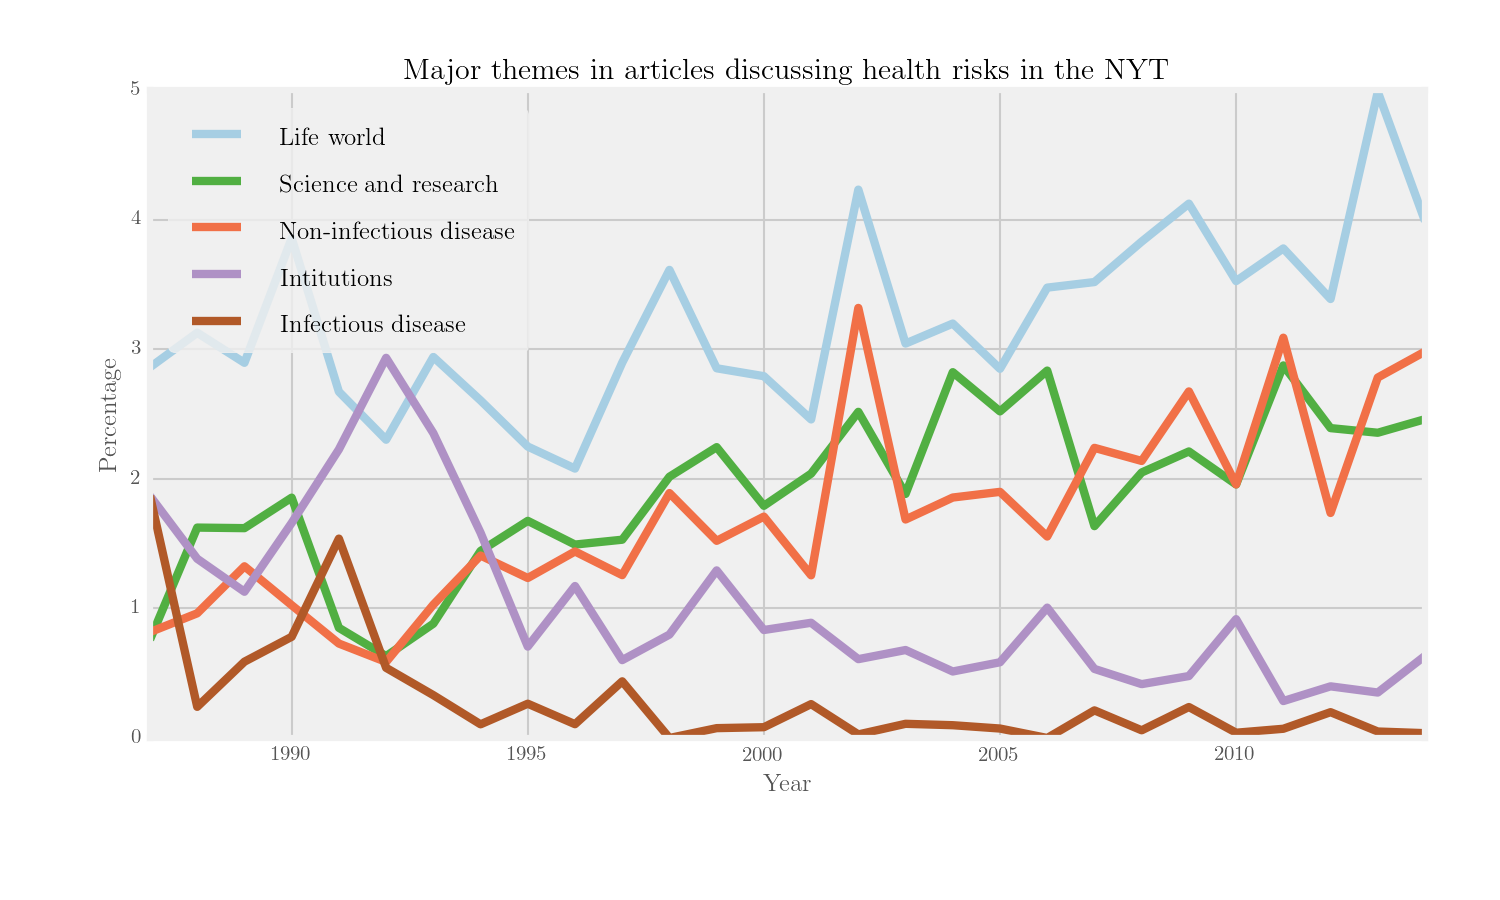
\includegraphics[width=0.75\textwidth]{../images/themes-health}}
\caption{Major themes (health subcorpus)}
%\label{fig:comparison}
\end{figure}

The overview shows the clear trend of decreasing reporting on infectious diseases and institutions related to the risk semantic in New York Times coverage. It also shows the risk of everyday life people referred to when using the risk semantic, the importance of science and research for driving the usage of the risk semantic as well as the non-infectious diseases such as cancer and life style diseases.

\section{Concluding remarks}

The analyses have shown a number of clear linguistic trends in media discourses utilising the risk semantic which indicate the growing institutionalisation of risk practices but can also be used to examine and test hypotheses from risk studies. 

Our data show an interesting ambivalence in the reporting of the NYT, similar to what was suggested in Beck's individualisation thesis (1992): A culture of institutional individualism takes place at a time when individuals can increasingly less control decision making outcomes. As a result we find a shift towards greater emphasis on everyday life social groups (e.g. women, men, children) in stories, but, at the same time, less agency in the linguistic expressions related to everyday people. Concurrently, the notion of risk calculation decreases, in favour of a general sense of exposure to risk. These results altogether support the assumption that in advanced modern societies all the advancement in science and technology---including medical technologies---has not supported discursive forms of control but discourses of uncertainty and potential risk. However, presentations differ regarding social groups. The emphasis on everyday life people in news coverage is increasing while it is mainly powerful people and organisations which are presented as decision makers. Everyday life people are usually presented as risk bearers in news reporting of the NYT.

There is also good evidence that risk words increasingly occur in the context of scientific studies as a technical term. This shows that the general trend Skolbekken (1995) observed in the 1980s and 1990s towards risk studies in medical sciences has found its way into media coverage. It also supports the view of Mairal (2011) that risk enters the media as part of a new, evidence-based genre of news reporting. 

We also found evidence that risk as a semantic process is in consistent decline, becoming steadily displaced by risk as a participant in discourse, or risk as a modifier of other kinds of processes and participants. In part, this is an expression of the institutionalisation of risk practices in social institutions, the kind of modifier on the sharpest upward trajectory is pre-head nominal modification---a form closely associated with occupations (e.g. \emph{financial risk managers}), organisations (e.g. \emph{risk budgeting}) or practices (e.g. \emph{risk arbitrage}). 

We were also able to show a number of clear trends in the health sector. Reporting of infectious diseases decreased after the AIDS crisis in the USA, while non-infectious diseases gain prominence alongside greater focus on terms for everyday people. This mainly reflects ongoing issues such as different forms of cancer and how to deal with it and the so called civilisation illnesses which tend to occupy more space in news coverage over decades.

Our research is only the beginning, at this point intended to determine whether we can find compelling linguistic evidence for institutional change in print news archives. Though our present analysis appears to have demonstrated that this is methodologically feasible, we have yet to triangulate our results with sustained, contextualised interpretation of individual texts within the corpus.

Accordingly, further research should focus on detailed qualitative institutional analysis, examining how discursive shifts in prototypical articles across the corpus are linked to specific institutional and socio-cultural changes. The increasing use of the \emph{at-risk} modifier, or the strong increase of the notion of the \emph{risk factor} (Zinn \& McDonald 2015), seems in different ways linked to broader social changes of the organisational regulation of the social. To re-construct this connection would allow a more fundamental understanding of how social and linguistic changes are connected.

We faced a number of difficulties. To begin with, the challenge of translating and connecting sociological thinking with corpus linguistic research strategies and elaborate functional grammars is by no means a simple task. Corpus linguistics, in seeking to distil the content of very large collections of text, may be at odds with a sociological tradition of sustained analysis of smaller, well-contextualised samples. Though the goal within the emerging field of corpus-assisted discourse studies is to use quantitative and qualitative methods as a methodological synergy (Baker et al, 2008), such a goal is difficult to operationalise when working with a very large corpus comprised of many subcorpora. Furthermore, shortcomings in the availability of digital tools for doing quantitative functional linguistic research mean that the accuracy and\slash or usefulness of software used to automatically annotate data remains a serious issue. CoreNLP's existing dependency parser, for example, does not distinguish grammatically between process-range configurations (She took a risk) and transitive processes (She took an apple), despite important differences in meaning. This limits what can be automatically located, or adds considerable complexity to the process of querying the corpus and manipulating the results.

Finally, systemic functional linguistics encompasses a theory of the relationship between text and context that in many respects clashes with mainstream sociological theory: the notion that context is in text is hard to reconcile with sociological analyses of texts that centre on highlighting relationships between texts and the broader social changes that may inform the production of texts, while leaving little trace in the lexical and grammatical choices made therein.

Though the analyses show results that are certainly an expression of broader social changes, there are a number of potential future avenues we hope to explore: comparison of newspapers by location, political orientation or language is indeed possible using the methods developed for this project, and may prove insightful Having more data available will also allow us to conduct more fine-grained analysis of developments in different social domains such as politics, economics, health, sports, and life world. On this basis we will start with comparative international analysis.

We are also particularly keen to engage with the question of how related terms such as danger, threat, chance and security relate to the identified shifts in health risk discourse. Sustained focus on particular kinds of health risks, such as cancer or obesity, could do much to elucidate longitudinal transitions toward or from risk. 








% ========== OLD CHAPTER ============


%\chapter{A comparison of economics, health, and political risks}

%In this chapter, we use subcorpora of economics, health and politics articles to understand how risk words change in specific semantic fields. Due to the smaller size of these subcorpora, as a general rule, the kinds of specific grammatical queries used in the previous chapter were not useful, as they generated very low numbers of results. Accordingly, this part of our investigation includes analyses of keywords and n-grams.

%\begin{figure}[htb!]
%\centering
%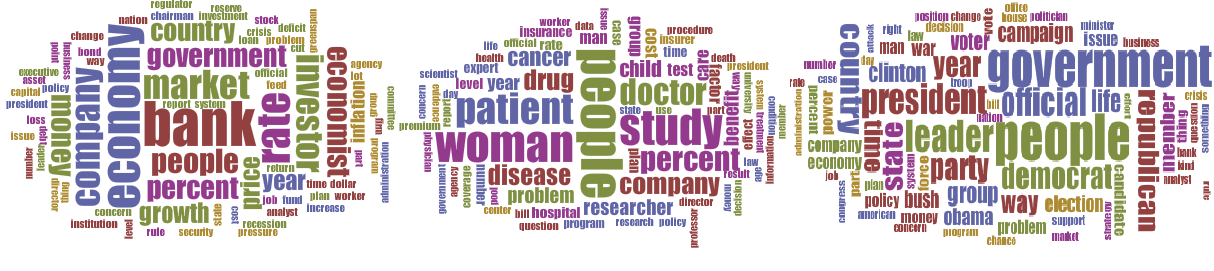
\includegraphics[width=0.70\textwidth]{../images/clouds.png}
%\caption{Key participants in the \emph{Economics}, \emph{Health} and \emph{Politics} subcorpora}
%\label{fig:clouds}
%\end{figure}

%\begin{figure}[htb!]
%\centering
%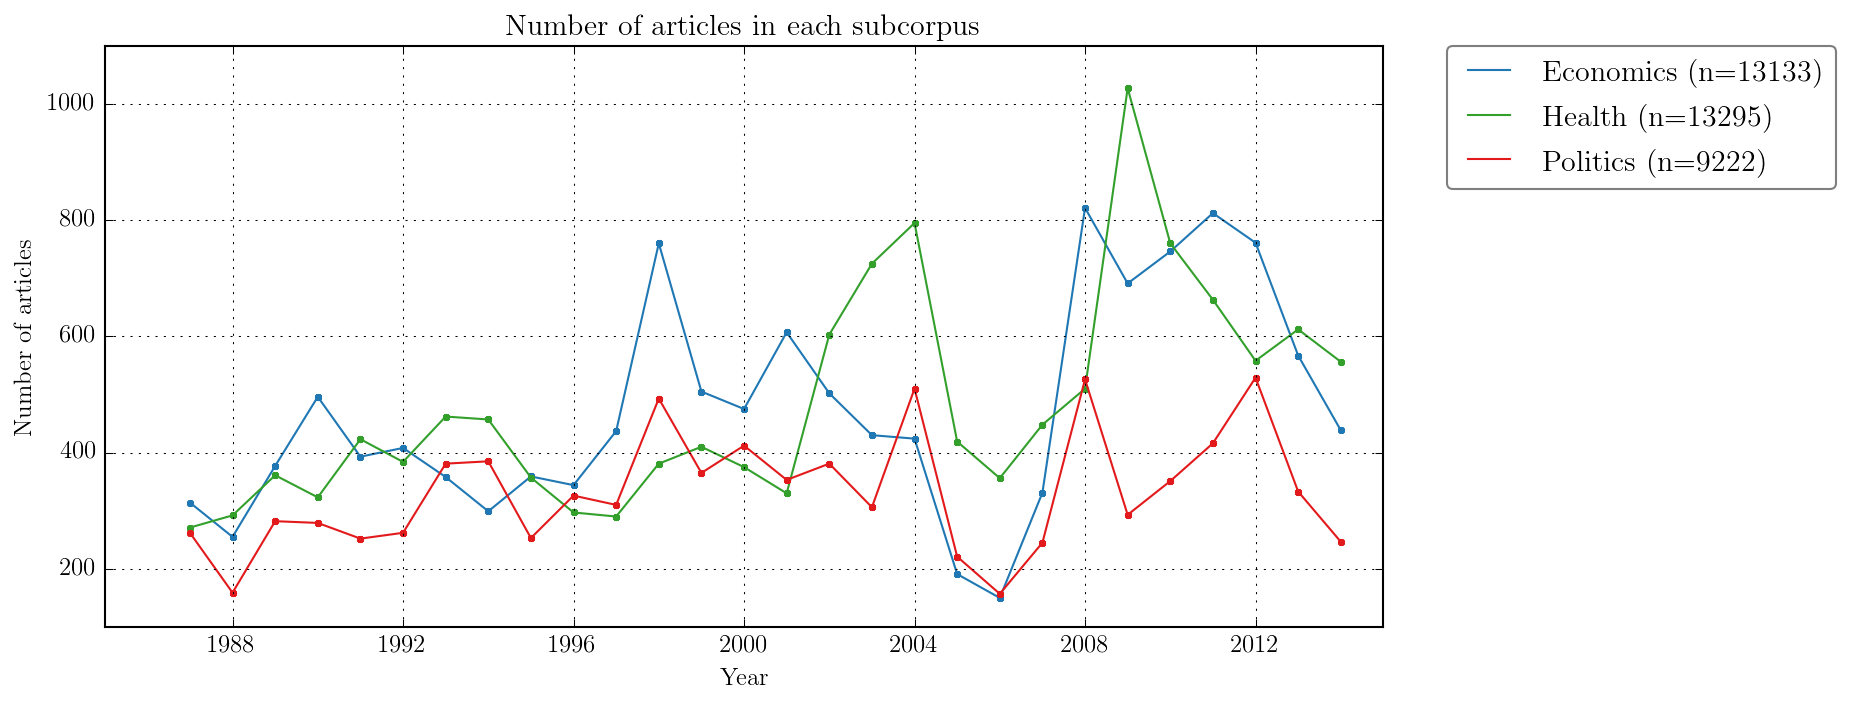
\includegraphics[width=.70\textwidth]{../images/number-of-articles-in-each-subcorpus.png}
%\caption{Number of articles in each subcorpus}
%\label{fig:article_per_subcorpus}
%\end{figure}

%%
%%Due to time constraints, we restricted the topic comparison to domains that had yielded interesting insights in the earlier interrogations. Further, we found that the smaller size of the subcorpora limited us to lexicogrammatical queries that outputted a large enough number of results for quantitative reliability. Thus, we focussed on the following three areas:

%\begin{table}[htb!]
%\centering
%\small
%\begin{tabular}{|l|l|l|}
%\hline
%\textbf{Economics}   & \textbf{Health}         & \textbf{Politics}     \\ \hline
%political   & high           & political    \\ \hline
%big         & great          & great        \\ \hline
%economic    & low            & big          \\ \hline
%financial   & other          & high         \\ \hline
%great       & serious        & own          \\ \hline
%high        & financial      & serious      \\ \hline
%more        & potential      & new          \\ \hline
%real        & medical        & real         \\ \hline
%systemic    & more           & considerable \\ \hline
%significant & significant    & more         \\ \hline
%new         & cardiovascular & other        \\ \hline
%little      & political      & significant  \\ \hline
%global      & possible       & economic     \\ \hline
%serious     & small          & financial    \\ \hline
%other       & real           & potential    \\ \hline
%excessive   & such           & personal     \\ \hline
%potential   & genetic        & little       \\ \hline
%such        & ovarian        & such         \\ \hline
%much        & same           & public       \\ \hline
%own         & bad            & military     \\ \hline
%\end{tabular}
%\caption{Most common adjectives modifying nominal risks in the topic subcorpora}
%\label{tab:echepo_adjmod}
% \end{table}

\chapter{\emph{Risk} in health articles in the NYT}

This chapter summarised the methods and results from an investigation of articles annotated as being about health topics. The work presented here is covered  in substantially more detail in our in-press chapter:  name?

\section{Methdological considerations when working with a smaller corpus}

Our topic subcorpora were much smaller than our main corpus. As a result, lexicogrammatical querying did not tend to yield quantitatively reliable results. Accordingly, other kinds of corpus linguistic investigation, not as reliant on grammatical structures, were applied. 

First, we considered \emph{keywords}---that is, words that were unusually frequent within the health corpus when compared to the corpus as as a whole. Linear regression was used to determine the slope of each keyword's trajectory over the length of the x-axis. Results were then sorted into two groups, based on the steepness of the incline\slash decline of the slope. Results whose slope significance was over 0.05 were automatically excluded.

\begin{figure}[htb!]
\centering
\begin{minipage}{.48\textwidth}
\centering
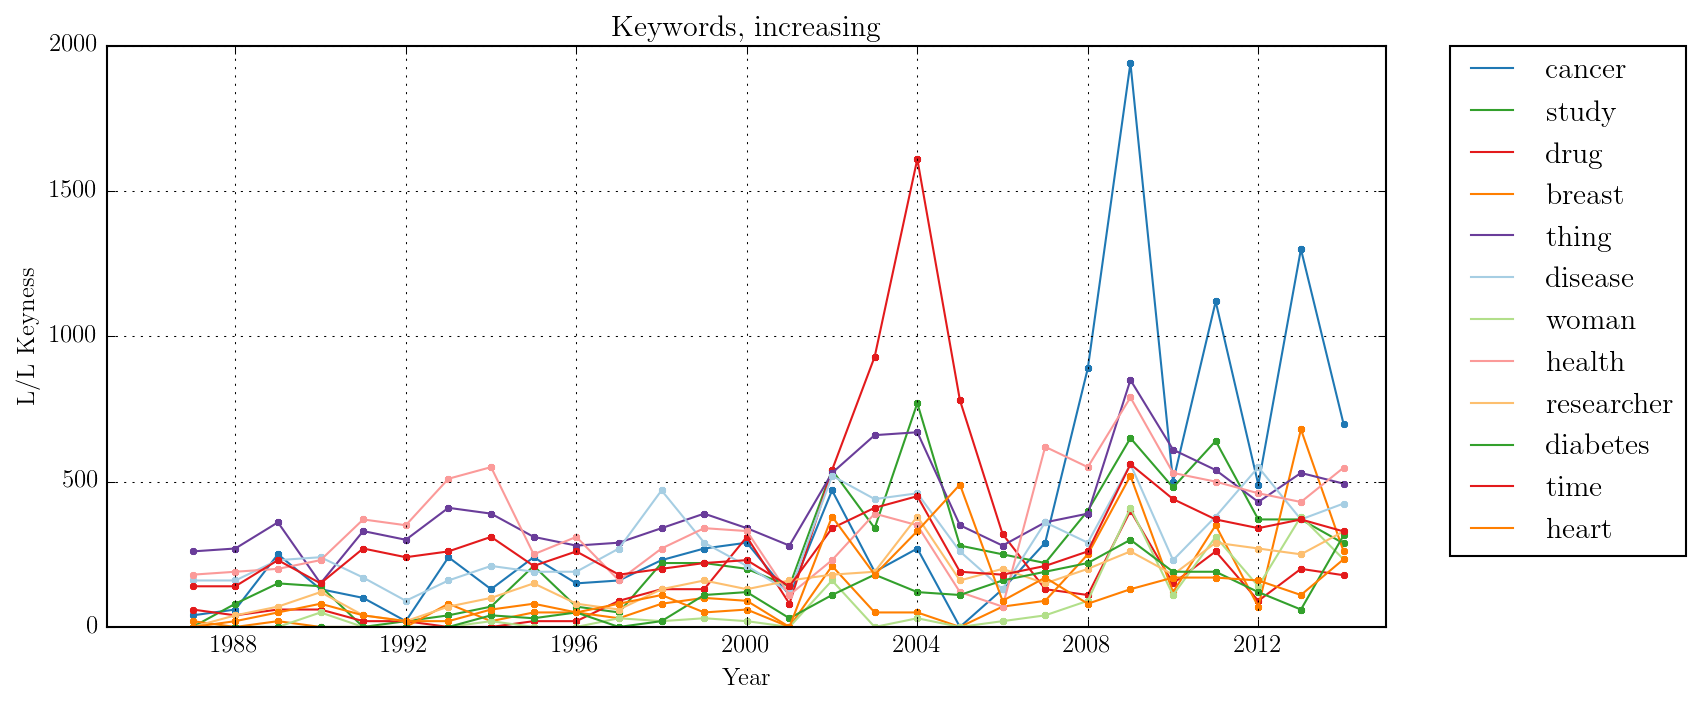
\includegraphics[width=.95\textwidth]{../images/keywords-increasing.png}
\caption{Keywords becoming more key over time}
\label{fig:key-inc}
\end{minipage}%
\begin{minipage}{.48\textwidth}
\centering
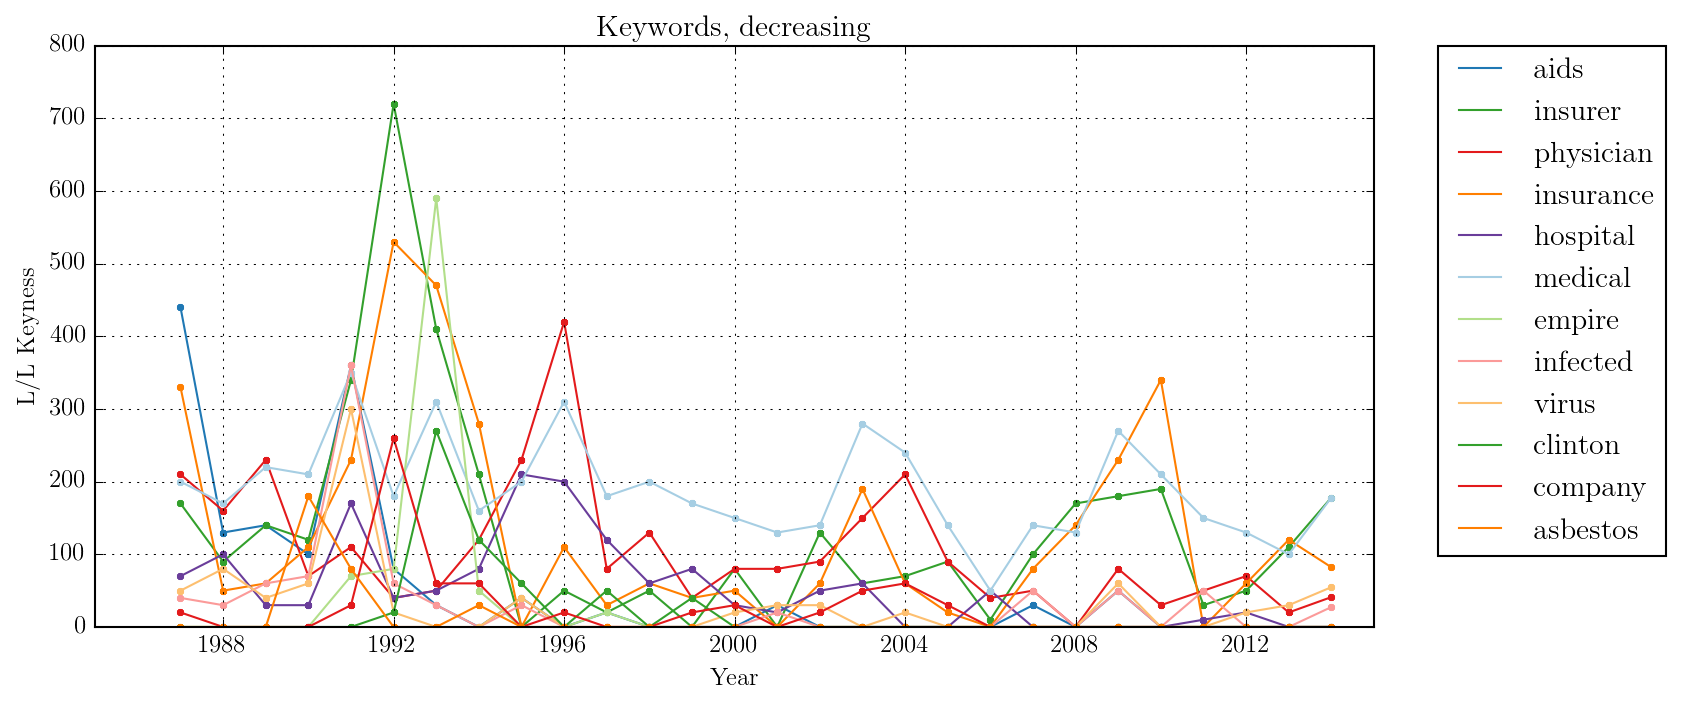
\includegraphics[width=.95\textwidth]{../images/keywords-decreasing.png}
\caption{Keywords becoming less key over time}
\label{fig:key-dec}
\end{minipage}
\end{figure}
%
Interestingly, words relating more closely to everyday life world concerns are increasing over time, while terms relating to healthcare institutions are decreasing.

Next, we were interested in \emph{bigrams}---that is, words that occur beside each other multiple times within a corpus. Bigrams containing a stopword were excluded from analysis, as these results were generally common clusters of closed class words (\emph{in the}, \emph{of a}, \emph{one day}, etc.). Again, linear regression was used to group results into increasing and decreasing groups.

\noindent
\begin{figure}[htb!]
\centering
\begin{minipage}{.42\textwidth}
\centering
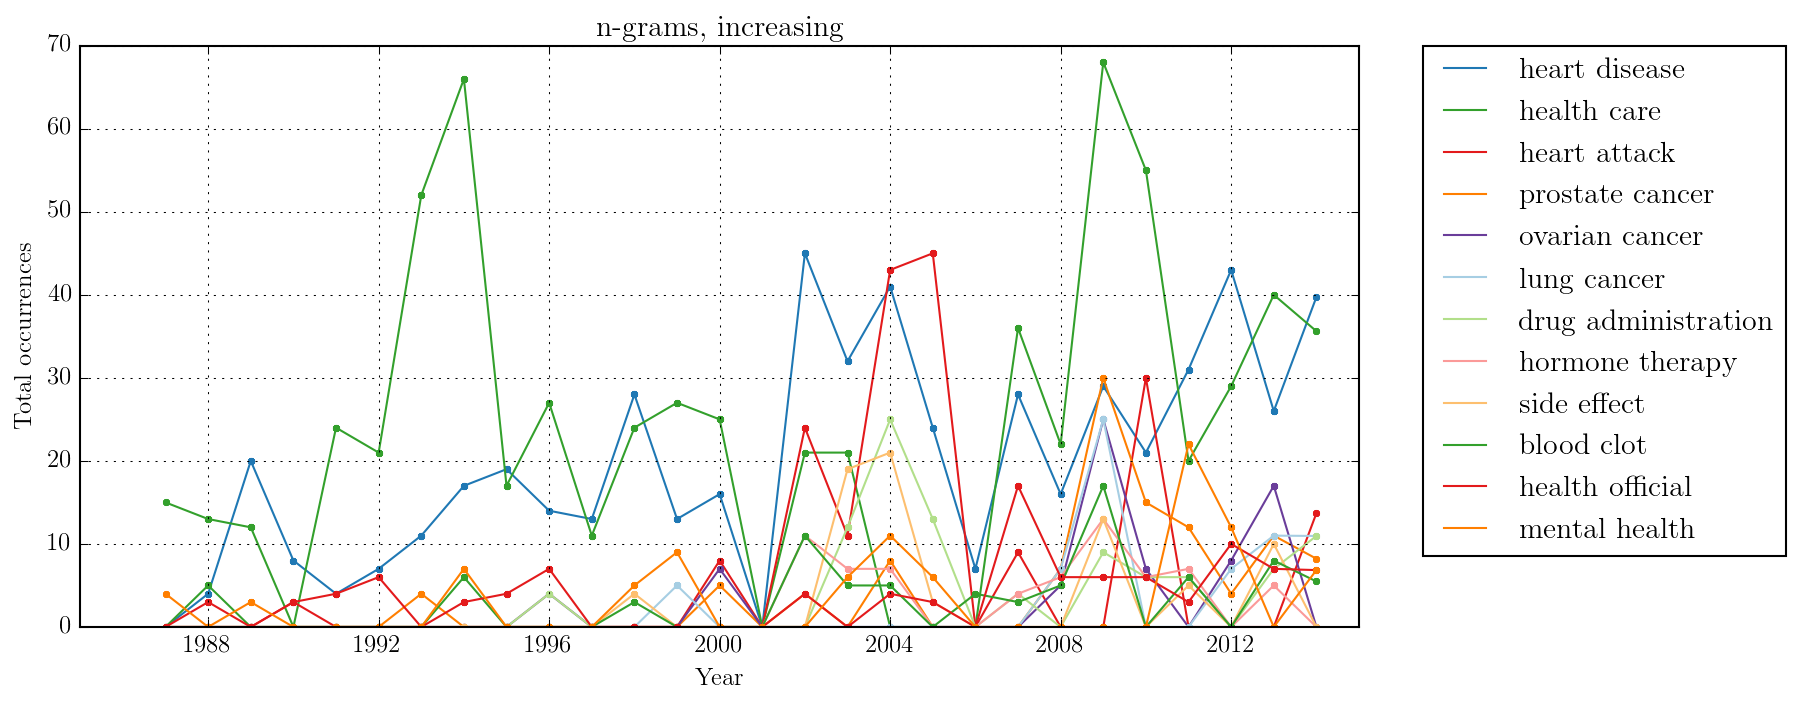
\includegraphics[width=1\textwidth]{../images/ngrams-increasing.png}
\caption{bi-grams becoming more frequent over time}
\label{fig:ngram-inc}
\end{minipage}%
\begin{minipage}{.42\textwidth}
\centering
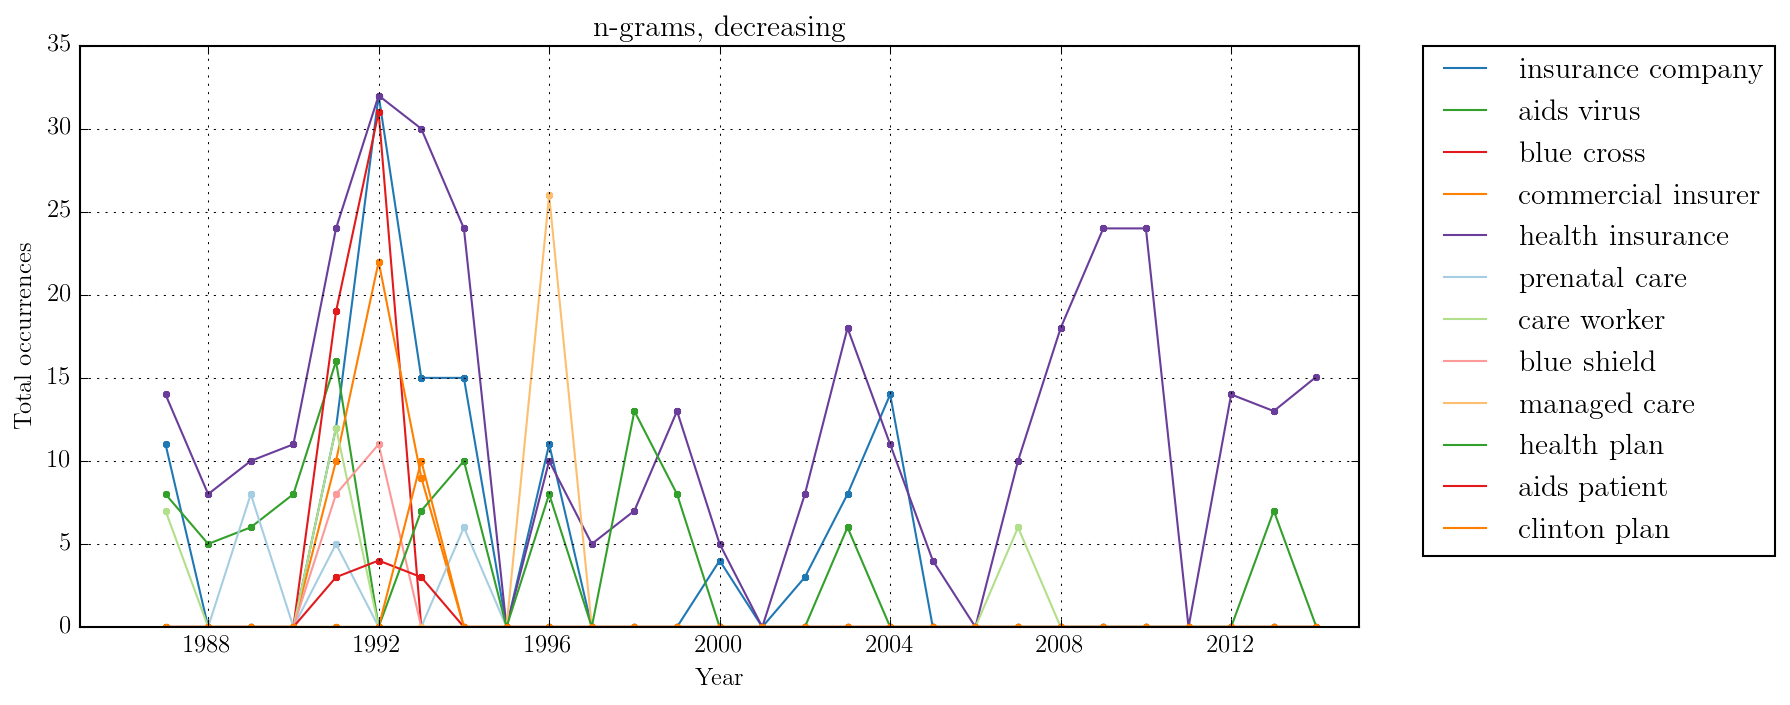
\includegraphics[width=1\textwidth]{../images/ngrams-decreasing.png}
\caption{bi-grams becoming less frequent over time}
\label{fig:ngram-dec}
\end{minipage}
\end{figure}

We grouped these into themes, with results entered into one or more categories. Ambiguous results were often concordanced in order to determine the main context of use: \emph{athlete}, for example, could indicate the health condition (\emph{Athlete's foot}), a chain of footwear stores, or denote athletes themselves. The latter was revealed to be by far the most common context, and athlete was thus added to \emph{People, everyday}.

\subsection{Nominal groups in the health subcorpus}

We also looked at key nouns, or nominal groups. By measuring the slope of trend lines, we could ascertain which groups were becoming more or less common.

\noindent
\begin{figure}[htb!]
\centering
\begin{minipage}{.42\textwidth}
\centering
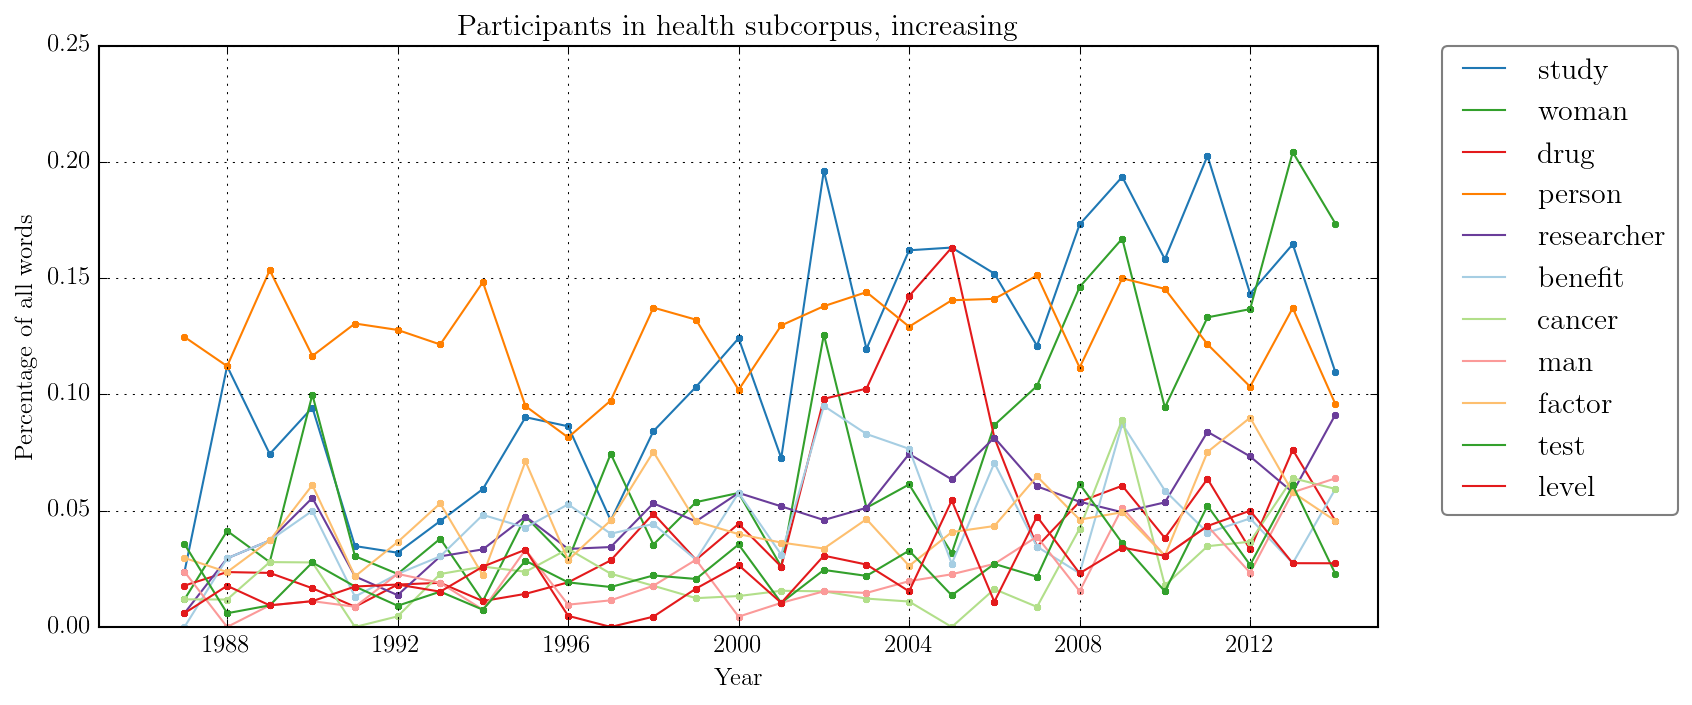
\includegraphics[width=1\textwidth]{../images/1.png}
\caption{Absolute frequency of nominal groups becoming more frequent over time}
\label{fig:1}
\end{minipage}%
\begin{minipage}{.42\textwidth}
\centering
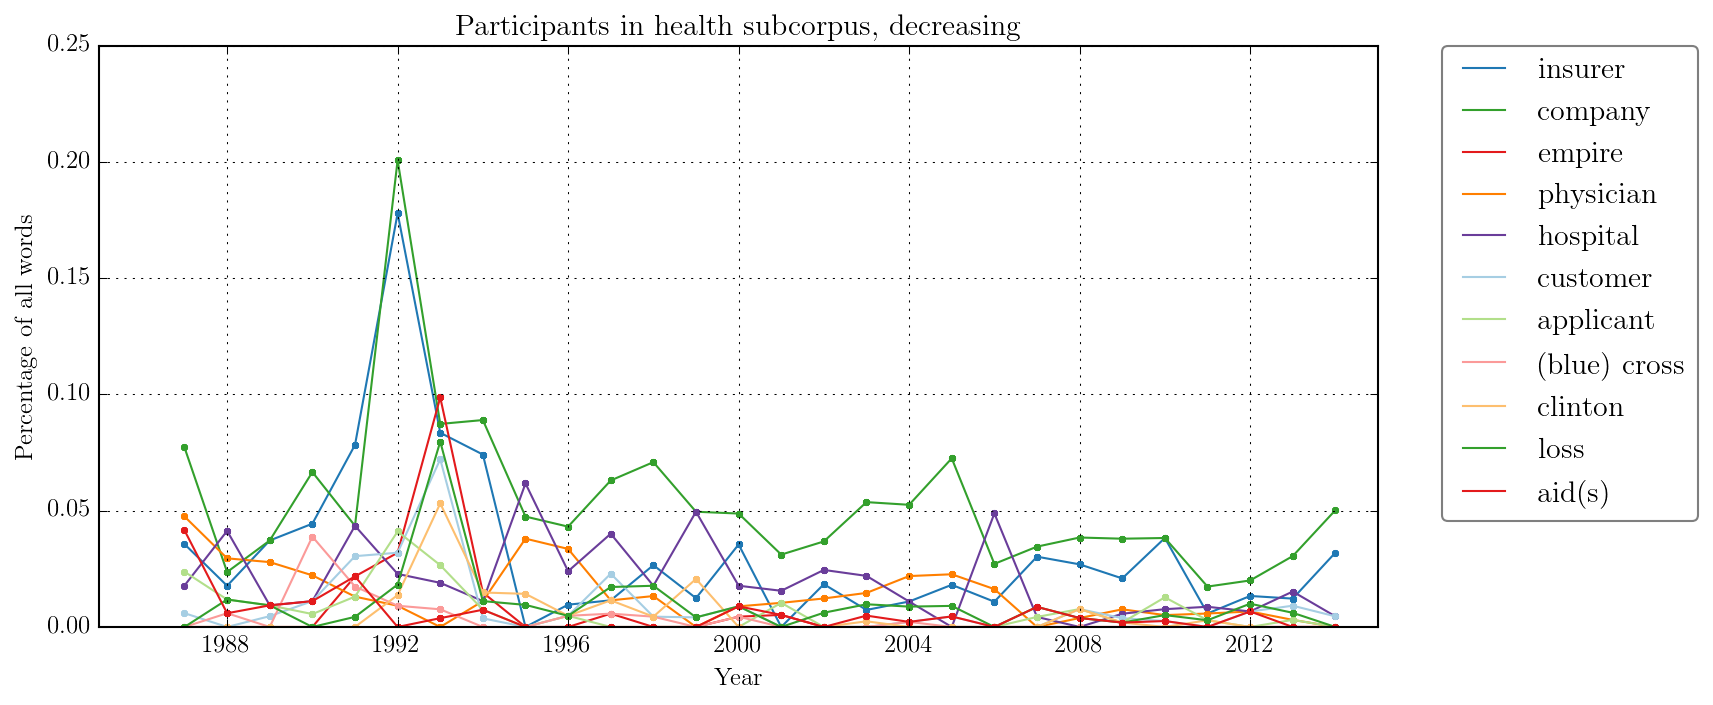
\includegraphics[width=1\textwidth]{../images/2.png}
\caption{Relative frequency of nominal groups becoming more frequent over time}
\label{fig:2}
\end{minipage}
\end{figure}
\noindent
\begin{figure}[htb!]
\centering
\begin{minipage}{.42\textwidth}
\centering
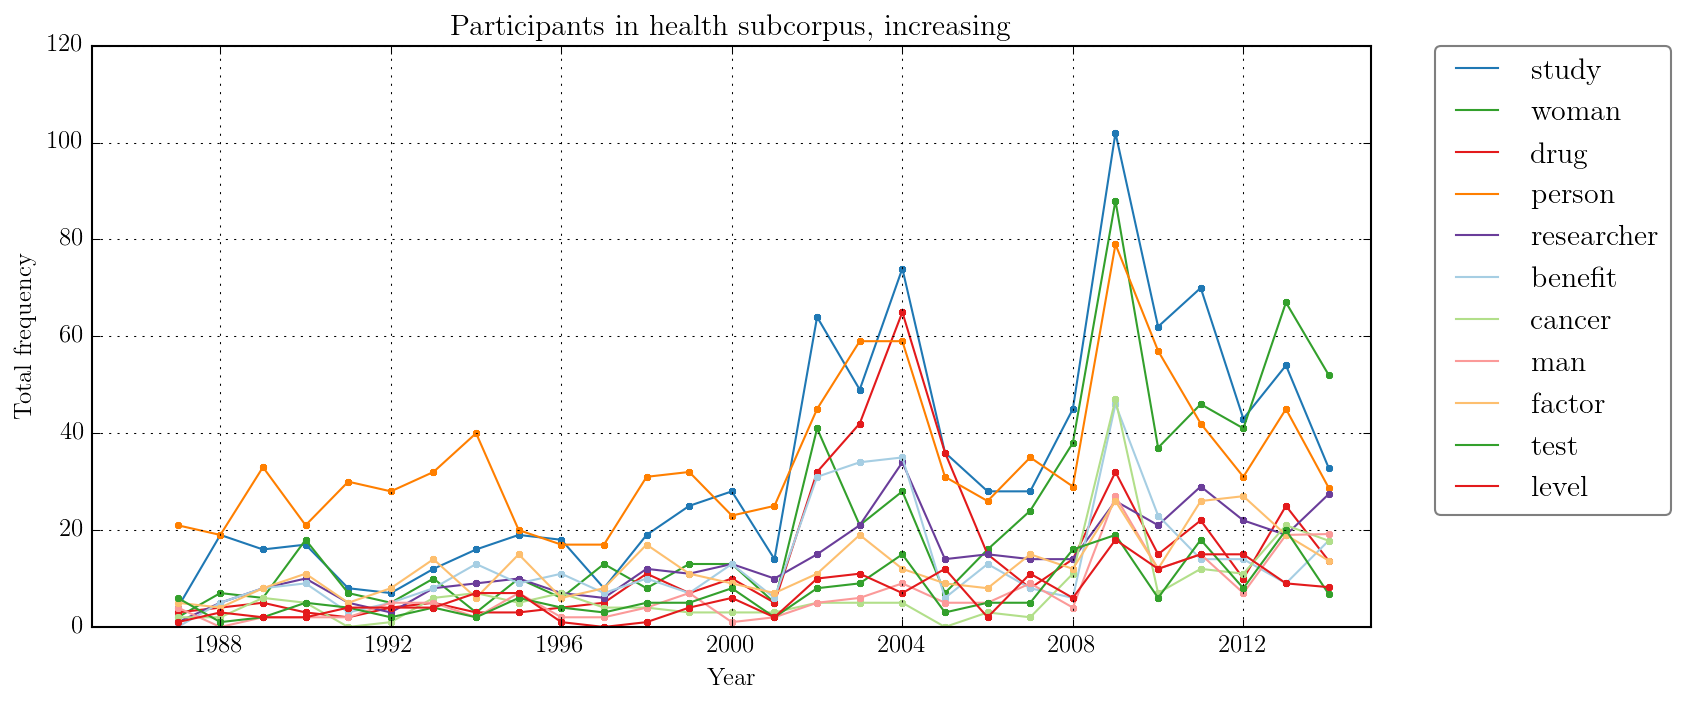
\includegraphics[width=1\textwidth]{../images/3.png}
\caption{Relative frequency of nominal groups becoming more frequent over time}
\label{fig:3}
\end{minipage}%
\begin{minipage}{.42\textwidth}
\centering
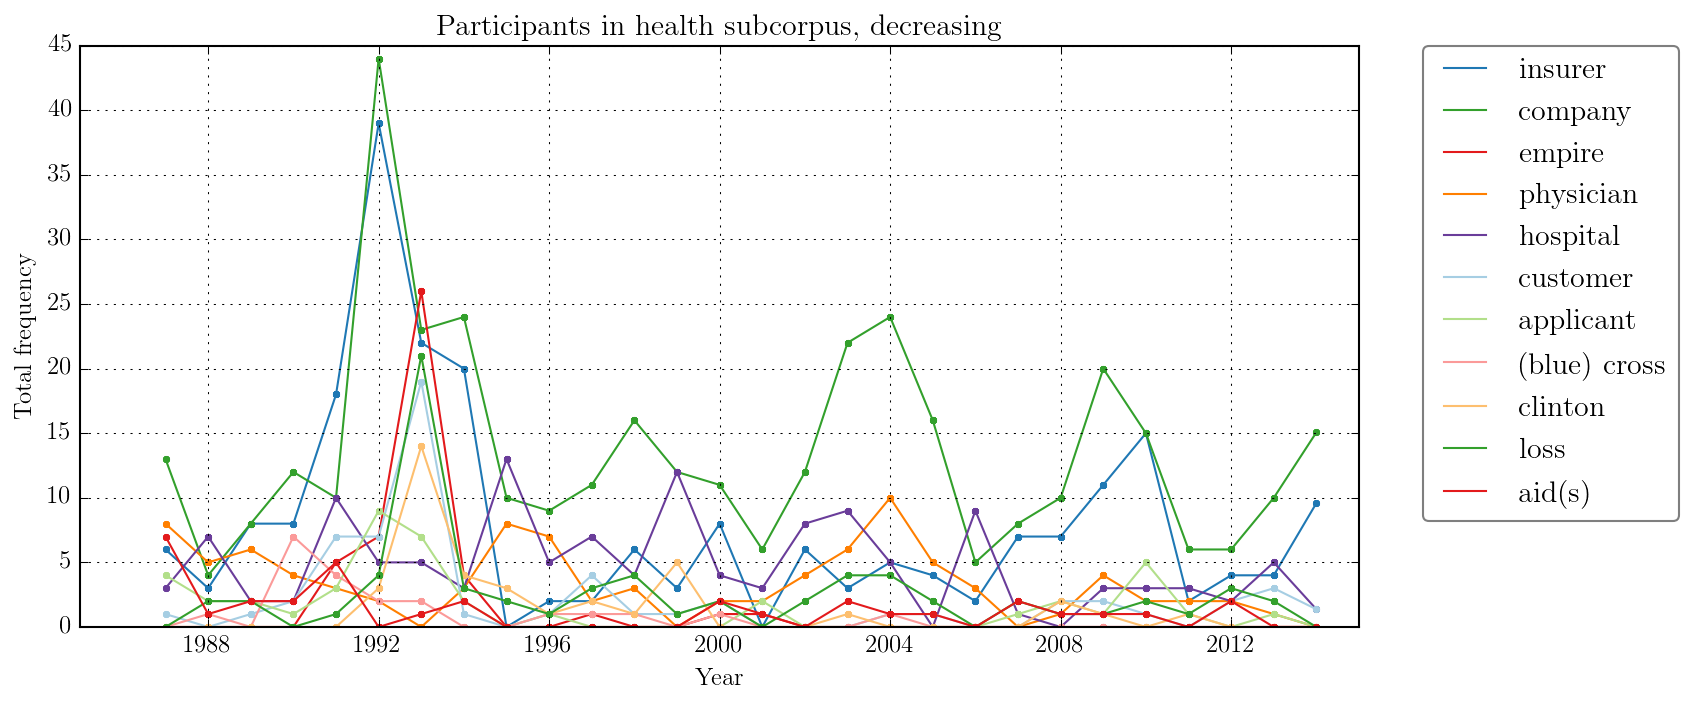
\includegraphics[width=1\textwidth]{../images/4.png}
\caption{Relative frequency of nominal groups becoming less frequent over time}
\label{fig:4}
\end{minipage}
\end{figure}


\begin{itemize}
\item The first major theme that emerges from this interrogation is the shift from infectious to non-infectious disease.
\item A second point of interest is the decline in terms related to insurance. Though the prevalence of health insurance in mid 1990s articles was unexpected, as it corresponds with Hillary Clinton's efforts to increase health insurance coverage in the USA, unexpected was the lack of an upswing in insurance terms during the pushes for healthcare reform throughout the Obama administration.
\item Also apparent is an upward trend for nominal groups related to research (\emph{study, percent, research, etc.}).This finding was of particular interest, given that the increasing contestation of academic and scientific research are core hypotheses made by Beck. Concordancing was used to look for evidence of contestation when the nominal groups related to research, researchers, studies, etc. were instantiated (see Table \ref{tab:researcher}).
\end{itemize}
%
Broadly speaking, institutional social actors, political representatives and the like appear to have been displaced by individual human actors and components within their everyday life world. The exception to this rule is the domain of research, which is becoming increasingly salient in health reporting. Though further investigation into the emergence of research as a key semantic domain within risk discourse is needed, we hypothesise that the increase is the cause of both institutional factors (the time- and cost-effectiveness of reporting on science) as well as sociological changes (an increased consciousness of science, etc.) The lack of contestation of research in the NYT, however, is at least partially at odds with Beck's conceptualisation of risk in reflexive modernity. Due to the fact that our data is from only one source, we cannot 

If contestation of science and research happens mostly within certain communicative genres (e.g. casual conversation, Tweets, etc.) or among certain demographics, it seems prudent to suggest further research focussing on the presentation of science within different kinds of talk. This could be useful in building an empirically driven account of the genesis, mechanism and effects of contestation of mainstream science and research.

\afterpage{%
\begin{table}
\centering
\tiny
\ttfamily
\begin{tabular}{lrrl}
1 & We know this now because                           & researchers & tested both theories , side by side , to see which \\
2 & something the public did not : Yale University     & researchers & had tentatively concluded that PPA was linked to a \\
3 & Instead ,                                          & researchers & say , young killers must be seen as extremely      \\
4 & of men with E.D. , or at risk for developing it ,  & researchers & in Italy found that the men could improve their    \\
5 & If you were an academic                            & researcher  & , you 'd have to persuade your institutional       \\
6 & Some                                               & researchers & believe hyperthymics may be at increased risk of   \\
7 & index , smoking and several other risk factors ,   & researchers & found that women on postmenopausal hormone therapy \\
8 & will have public health consequences , the         & researchers & said                                               \\
9 & Finally , and perhaps most powerfully ,            & researchers & say that a life in poverty is a life of stress     \\
10 & Office of Protection from Research Risks said the  & researchers & altered the medical records of patients , then     \\
11 & In their paper , the                               & researchers & noted that `` countries in which wine is the       \\
12 & In another study , by                              & researchers & at the University of Connecticut , leg strength    \\
13 & In an unexpected finding , the                     & researchers & reported that the women receiving goserelin also   \\
14 & that , far from protecting the heart as many       & researchers & had assumed , the therapy may have put the women   \\
15 & Now                                                & researchers & have found that elevated risk of psychiatric       \\
16 & of a New York Fire Department rescue company and a & researcher  & who is exploring the psychological bases of        \\
17 & Department of Veterans Affairs said the California & researchers & did not properly assess the safety of experimental \\
18 & Other                                              & researchers & , working with similar kinds of data , have        \\
19 & The                                                & researchers & concluded that the study '' provides the first     \\
20 & On the other hand , said Dr. Susan Czajkowski , a  & researcher  & at the National Heart , Lung and Blood Institute   \\
21 & exactly how a given AIDS patient was infected ,    & researchers & do not know exactly how much the risk of           \\
22 & In an effort to finance debts , '' the             & researchers & said , `` ordinary people are paying the ultimate  \\
23 & during the next 25 years of about 6 percent , the  & researchers & found                                              \\
24 & To obtain consent ,                                & researchers & are required to explain that the experiments are   \\
25 & slightly increasing their risks of dying earlier , & researchers & reported yesterday                                 \\
26 & Utah                                               & researchers & have videotaped 150 couples to measure the effect  \\
27 & blood cells -- became patients ' property ,        & researchers & taking them without detailed consent and explicit  \\
28 & In mapping the human genome ,                      & researchers & determined that nearly 99 percent of genetic       \\
29 & The                                                & researchers & were unable to include family history of diabetes  \\
30 & of Internal Medicine , Dr. Solomon and other       & researchers & looked at the comparative risks posed by different \\
31 & the perception of risk , said Pete Delaney , a     & researcher  & with the administration , adding that only about 9 \\
32 & The                                                & researchers & conclude that irregular sleep by itself may be a   \\
33 & Dr. Bernard H. Fox , a federal                     & researcher  & who became a pioneer in investigating the effect   \\
34 & The                                                & researchers & said it was unclear why smoking appeared to        \\
35 & The Stanford                                       & researchers & , who included Dr. Irving Weissman , a leading     \\
36 & But                                                & researchers & like Dr. Monahan and Dr. McNiel are applying       \\
37 & A study of 1,240 people by                         & researchers & at Case Western Reserve University in Cleveland    \\
38 & that of diabetes , '' said Dr. Steven G. Deeks , a & researcher  & at the University of California , San Francisco    \\
39 & In addition ,                                      & researchers & hope that the studies linking the disorder to      \\
40 & night on WNBC-TV , that Cornell University         & researchers & have found a risk of alcoholism among New York     \\
41 & , suggesting chance could play a role , but        & researchers & say the trends are credible because they are       \\
42 & The                                                & researchers & also found that patients became significantly less \\
43 & Over all ,                                         & researchers & found that calcium supplements did not lower the   \\
44 & of the power AIDS activists have mustered to push  & researchers & to do experiments that many experts deem foolish   \\
45 & The                                                & researchers & next study the extent to which medical treatment   \\
46 & was the fourth-leading risk factor for death , the & researchers & said                                               \\
47 & study 's author , Kathleen Miller , an addiction   & researcher  & at the University of Buffalo , says it suggests    \\
48 & The                                                & researchers & claim that the benefits of the research -- greater \\
49 & Some                                               & researchers & suspect genetics : Maybe thin people who develop   \\
50 & Dr. Bishop and Dr. Varmus , along with other       & researchers & , have found that the genes can cause cancer in    \\
51 & Finally ,                                          & researchers & at Tufts reported last month in The Journal of     \\
52 & The lead                                           & researcher  & , Dr. Tina V. Hartert , director of the Center for \\
53 & harmful cholesterol in the blood , even when the   & researchers & accounted for other risk factors for high          \\
54 & on cases stemming from the Sept. 11 attacks ,      & researchers & found that the more deeply therapists were         \\
55 & The                                                & researchers & did find an increased risk of other , less common  \\
56 & The inquiry in Ms. Wan 's case found that          & researchers & had adequately explained the risks to her and that \\
57 & For example , she said ,                           & researchers & are experimenting with fast-growing carp that      \\
58 & than 23,000 Greek men and women ages 20 to 86 ,    & researchers & found that napping at least three times a week for \\
59 & precision afforded by simple computing devices ,   & researchers & say , promise to deliver new insights on risk      \\
60 & only two categories of risk , minimal and great ,  & researchers & were often discouraged from doing research         \\
61 & the clear advantage of moderate drinking , the     & researchers & presented their findings with strong caveats       \\
62 & As the genes become better understood ,            & researchers & expect to find ways to block them if they become   \\
63 & adolescents followed over a period of nine years , & researchers & at the New York Psychiatric Institute found that   \\
64 & Health , for example , said that 100 psychiatric   & researchers & gathered in a room would all probably agree that   \\
65 & smoking might have damaged the fathers ' sperm ,   & researchers & said yesterday                                     \\
66 & with 20 percent of the control group , the         & researchers & found                                              \\
67 & The                                                & researchers & found that for each four-inch increase in height   \\
68 & between height and cancer may help guide           & researchers & to study hormones and growth factors that          \\
69 & Why do                                             & researchers & and willing patients test the boundaries of        \\
70 & 's disease as those who have never smoked ,        & researchers & say , and several small studies have indicated     \\
71 & But                                                & researchers & said they had never seen this before , either in   \\
72 & In 2012 , British                                  & researchers & , by combining results from clinical trials that   \\
73 & After adjusting for various health factors , the   & researchers & found that for each increase of 10 micrograms per  \\
74 & The F.D.A. has asked                               & researchers & at Columbia to reclassify the cases of self-harm   \\
75 & The                                                & researchers & said this was troubling , given recent studies     \\
76 &  A large team of                                    & researchers & , led by V. Wendy Setiawan , an assistant          \\
77 &  and violated Federal regulations because the       & researchers & had not informed patients of the risks             \\
78 &  Yet                                                & researchers & also concluded the risk of stroke was the same as  \\
79 &  In 2002 ,                                          & researchers & halted the largest clinical trial ever conducted   \\
80 &  , and while they might not be surprising to        & researchers & , they were intended to inform the public as well  \\
81 &  Many                                               & researchers & said anger-prone people could reduce the risk of   \\
82 &  Using preserved blood samples of pregnant women ,  & researchers & have found that low vitamin D levels are           \\
83 &  And so now                                         & researchers & have been working on new strategies : Developing   \\
84 &  This month , Danish                                & researchers & reported on a 15-year study of 12,000 nurses       \\
85 &  She said                                           & researchers & thought older medicine was riskier because the     \\
86 &  Last Sunday ,                                      & researchers & released data that showed that outdoor air         \\
87 &  But when the company and the                       & researcher  & are one and the same , he said , that check is     \\
88 &  Huntington 's disease and cystic fibrosis , and    & researchers & say tests identifying those at high risk of heart  \\
89 &  may increase with a father 's advancing age ,      & researchers & reported yesterday                                 \\
90 &  Denise Juliano-Bult , a                            & researcher  & at the National Institute of Mental Health , said  \\
91 &  those who gain fat around the hips and thighs ,    & researchers & say                                                \\
92 &  in the British Medical Journal in August ,         & researchers & in Argentina showed that women who were given      \\
93 &  Next ,                                             & researchers & said , they want to do a large study like one      \\
94 &  The                                                & researchers & noted that the drinks contain high levels of       \\
95 &  The                                                & researchers & offered some other examples of how the risks       \\
96 &  Some other                                         & researchers & questioned the findings , and most agreed that the \\
97 &  For purposes of comparison , the                   & researchers & also examined inherited variations in 13 genes     \\
98 &  And the flaws are compounded , the                 & researchers & said , when journalists do n't report the context  \\
99 &  A few years ago , Mercedes Carnethon , a diabetes  & researcher  & at the Feinberg School of Medicine at Northwestern \\
100 &  As with beta carotene ,                            & researchers & were shocked                                       \\
\end{tabular}
\caption{100 random instances of \emph{researcher} in the health subcorpus}
\label{tab:researcher}
\end{table}
\clearpage
}

\subsubsection{Beck's notion of increasingly contested science}

Key to Beck's notion of Reflexive Modernity is the idea that people confront and contest the science that brought about modernisation via the industrial revolution, as the negative repercussions of this science and modernisation witnessed first-hand (through pollution, etc.) \cite{ross_science_1996}. 

We found strikingly little evidence for contestation of scientific\slash academic research in the NYT. As can be seen in Table \ref{tab:researcher}, research and researchers are typically presented in a neutral light, with no explicit scepticism of their methods or findings. This is interesting, given that authors of many other kinds of writing, such as academic and fiction, have embraced the critical turn of scientific method against itself, under the banner of post-structuralism. Why not print journalism?

Many explanations are possible. Before we turn to them, it is important to remember that the representation of research in the NYT may be influenced by a number of independent factors. Foremost, it should be noted that print journalism centred on science is increasingly common. It is affordable, as the journalist does not need to investigate or travel in order to access the content, and much of the article body can consist of quotations from the journal article. It is also deemed reliable, having in many cases already been through peer-review. Given the rapid rise in the number of academic journals, as well as the increased ability to access these journals via the Web, increased reporting of academic research is perhaps an expected finding. 

Of more interest to us is the lack of scepticism. One possible explanation for this is that the NYT might not be the genre in which the contestation occurs. The absence of scepticism toward modern medicine, the pharmaceutical industry does not indicate that there is little scepticism toward these things in society in general. As reasons underlying this scepticism are often subjective and emotional, rather than empirically derived, it makes sense that such discourse would be more common in everyday conversations, for example, than in new journalism. While it is possible that such scepticism is mostly represented in Opinion and Editorial articles in the NYT, such articles comprise only a small fraction of all articles. Further research here would build corpora of different article types, and investigate how health discourse differs by the genre\slash section of the newspaper.

Another possible argument is that print news and modernity have a more-or-less symbiotic relationship. Indeed, the rise of print journalism closely parallels modernisation and industrialisation. The production and transmission of newspapers themselves is in many respects reliant upon technology popularised during industrialisation.

% The inability of science alone to solve conflicts and debates may be so, but this has little bearing on the usefulness of scientific research within print journalism. Journalism is not typically seeking to resolve, but merely to elucidate, sources of conflict and tension in the world at large.

% We should also note here that the emergence of science reporting does not necessarily mean than non-scientifically informed medical practice is being displaced:

\section{Methodological challenges during the health corpus investigation}

A major issue was the smaller size of the corpus, which necessitated different kinds of analysis. Within keywording and n-gramming, it became clear that broader linguistic change and specific events are difficult to separate. This, however, is where we can see the clearest examples of the link between events and language change. Interspersed throughout the keywords and n-grams are terms ranging in specificity. It is through taxonomisation and categorisation of these varying levels that we can hopefully smooth out our understnading of the influence of specific events on the risk semantic.\endnote{Since finalisation of this report, we have expanded on \texttt{corpkit}'s ability to process keywords in particular: documentation of preliminary findings is available at \url{https://www.github.com/interrogator/corpkit}.}

A second major challenge was an original project aim, to compare risk language in politics, health and economics articles. Despite a number of interrogations of this corpus, we have found the issue of working with three corpora, each containing almost thirty subcorpora, unmanageably complex. Though code can quickly iterate through each corpus, even taking advantage of parallel processing, constructing meaningful discussion of risk 

The huge amount of data and variables necessitates an additional stratum of distance from the texts themselves, and this distance leads to uncertainty in discussions about how and why risk language is changing. To grapple with this issue in the future, we envision a three-pronged approach:

\begin{enumerate}
\item Create more sophisticated code and methods, which can point to interesting phenomena within datasets quickly and accurately
\item Increase the time spent on contexutalised, qualitative analysis
\item Describe in more detail the media production climate and its role in news language
\end{enumerate}

\section{Summary}

The smaller size of health subcorpus necessitated different kinds of analysis. Fortunately, such methods are well-documented within corpus assisted discourse studies. Following on from these methodologies, we located particularly frequent terms, and analysed them in their context of use. Patterns quickly emerged: the domains of insurance, politics and infectious disease decrease in frequency over time, while non-infectious\slash lifestyle illnesses, everyday people and science\slash research became more prominent. Though of work on description of health risk in news media is far from complete, we believe we have demonstrated the fruitfulness of combining sophisticated programming concepts with mainstay social science methods such as thematic categorisation.
